% See https://chatgpt.com/share/673b30a9-1820-8000-90b6-c7f6e955bd6e
\documentclass[10pt,compress,t,notes=noshow, xcolor=table]{beamer}

\usepackage[]{graphicx}
% graphicx is loaded via lmu-lecture.sty as well
\usepackage[]{color}
% maxwidth is the original width if it is less than linewidth
% otherwise use linewidth (to make sure the graphics do not exceed the margin)
\makeatletter
\def\maxwidth{ %
  \ifdim\Gin@nat@width>\linewidth
    \linewidth
  \else
    \Gin@nat@width
  \fi
}
\makeatother

% ---------------------------------%
% latex-math dependencies, do not remove:
% - mathtools
% - bm
% - siunitx
% - dsfont
% - xspace
% ---------------------------------%

%--------------------------------------------------------%
%       Language, encoding, typography
%--------------------------------------------------------%

\usepackage[english]{babel}
\usepackage[utf8]{inputenc} % Enables inputting UTF-8 symbols
% Standard AMS suite (loaded via lmu-lecture.sty)
\usepackage{amsmath,amsfonts,amssymb}

% Font for double-stroke / blackboard letters for sets of numbers (N, R, ...)
% Distribution name is "doublestroke"
% According to https://mirror.physik.tu-berlin.de/pub/CTAN/fonts/doublestroke/dsdoc.pdf
% the "bbm" package does a similar thing and may be superfluous.
% Required for latex-math
\usepackage{dsfont}

% bbm – "Blackboard-style" cm fonts (https://www.ctan.org/pkg/bbm)
% Used to be in common.tex, loaded directly after this file
% Maybe superfluous given dsfont is loaded
% TODO: Check if really unused?
% \usepackage{bbm}

% bm – Access bold symbols in maths mode - https://ctan.org/pkg/bm
% Required for latex-math, preferred over \boldsymbol
% https://tex.stackexchange.com/questions/3238/bm-package-versus-boldsymbol
\usepackage{bm}

% pifont – Access to PostScript standard Symbol and Dingbats fonts
% Used for \newcommand{\xmark}{\ding{55}, which is never used
% aside from lecture_advml/attic/xx-automl/slides.Rnw
% \usepackage{pifont}

% Quotes (inline and display), provdes \enquote
% https://ctan.org/pkg/csquotes
\usepackage{csquotes}

% Adds arg to enumerate env, technically superseded by enumitem according
% to https://ctan.org/pkg/enumerate
% Replace with https://ctan.org/pkg/enumitem ?
% Even better: enumitem is not really compatible with beamer and breaks all sorts of things
% particularly the enumerate environment. The enumerate package also just isn't required
% from what I can tell so... don't re-add it I guess?
% \usepackage{enumerate}

% Line spacing - provides \singlespacing \doublespacing \onehalfspacing
% https://ctan.org/pkg/setspace
% \usepackage{setspace}

% mathtools – Mathematical tools to use with amsmath
% https://ctan.org/pkg/mathtools?lang=en
% latex-math dependency according to latex-math repo
\usepackage{mathtools}

% Maybe not great to use this https://tex.stackexchange.com/a/197/19093
% Use align instead -- TODO: Global search & replace to check, eqnarray is used a lot
% $ rg -f -u "\begin{eqnarray" -l | grep -v attic | awk -F '/' '{print $1}' | sort | uniq -c
%   13 lecture_advml
%   14 lecture_i2ml
%    2 lecture_iml
%   27 lecture_optimization
%   45 lecture_sl
\usepackage{eqnarray}

% For shaded regions / boxes
% Used sometimes in optim
% https://www.ctan.org/pkg/framed
\usepackage{framed}

%--------------------------------------------------------%
%       Cite button (version 2024-05)
%--------------------------------------------------------%
% Note this requires biber to be in $PATH when running,
% telltale error in log would be e.g. Package biblatex Info: ... file 'authoryear.dbx' not found
% aside from obvious "biber: command not found" or similar.
% Tried moving this to lmu-lecture.sty but had issues I didn't quite understood,
% so it's here for now.

\usepackage{textcase} % for \NoCaseChange
\usepackage{hyperref}

% Only try adding a references file if it exists, otherwise
% this would compile error when references.bib is not found
\IfFileExists{references.bib} {
  \usepackage{usebib}
  \usepackage[backend=biber, style=authoryear]{biblatex}

  \addbibresource{./references.bib}
  \bibinput{references}
}

\newcommand{\citelink}[1]{%
\NoCaseChange{\resizebox{!}{9pt}{\protect\beamergotobutton{\href{\usebibentry{\NoCaseChange{#1}}{url}}{\begin{NoHyper}\cite{#1}\end{NoHyper}}}}}%
}

%--------------------------------------------------------%
%       Displaying code and algorithms
%--------------------------------------------------------%

% Reimplements verbatim environments: https://ctan.org/pkg/verbatim
% verbatim used sed at least once in
% supervised-classification/slides-classification-tasks.tex
% Removed since code should not be put on slides anyway
% \usepackage{verbatim}

% Both used together for algorithm typesetting, see also overleaf: https://www.overleaf.com/learn/latex/Algorithms
% algorithmic env is also used, but part of the bundle:
%   "algpseudocode is part of the algorithmicx bundle, it gives you an improved version of algorithmic besides providing some other features"
% According to https://tex.stackexchange.com/questions/229355/algorithm-algorithmic-algorithmicx-algorithm2e-algpseudocode-confused
\usepackage{algorithm}
\usepackage{algpseudocode}

%--------------------------------------------------------%
%       Tables
%--------------------------------------------------------%

% multi-row table cells: https://www.namsu.de/Extra/pakete/Multirow.html
% Provides \multirow
% Used e.g. in evaluation/slides-evaluation-measures-classification.tex
\usepackage{multirow}

% colortbl: https://ctan.org/pkg/colortbl
% "The package allows rows and columns to be coloured, and even individual cells." well.
% Provides \columncolor and \rowcolor
% \rowcolor is used multiple times, e.g. in knn/slides-knn.tex
\usepackage{colortbl}

% long/multi-page tables: https://texdoc.org/serve/longtable.pdf/0
% Not used in slides
% \usepackage{longtable}

% pretty table env: https://ctan.org/pkg/booktabs
% Is used
% Defines \toprule
\usepackage{booktabs}

%--------------------------------------------------------%
%       Figures: Creating, placing, verbing
%--------------------------------------------------------%

% wrapfig - Wrapping text around figures https://de.overleaf.com/learn/latex/Wrapping_text_around_figures
% Provides wrapfigure environment -used in lecture_optimization
\usepackage{wrapfig}

% Sub figures in figures and tables
% https://ctan.org/pkg/subfig -- supersedes subfigure package
% Provides \subfigure
% \subfigure not used in slides but slides-tuning-practical.pdf errors without this pkg, error due to \captionsetup undefined
\usepackage{subfig}

% Actually it's pronounced PGF https://en.wikibooks.org/wiki/LaTeX/PGF/TikZ
\usepackage{tikz}

% No idea what/why these settings are what they are but I assume they're there on purpose
\usetikzlibrary{shapes,arrows,automata,positioning,calc,chains,trees, shadows}
\tikzset{
  %Define standard arrow tip
  >=stealth',
  %Define style for boxes
  punkt/.style={
    rectangle,
    rounded corners,
    draw=black, very thick,
    text width=6.5em,
    minimum height=2em,
    text centered},
  % Define arrow style
  pil/.style={
    ->,
    thick,
    shorten <=2pt,
    shorten >=2pt,}
}

%--------------------------------------------------------%
%       Beamer setup and custom macros & environments
%--------------------------------------------------------%

% Main sty file for beamer setup (layout, style, lecture page numbering, etc.)
% For long-term maintenance, this may me refactored into a more modular set of .sty files
\usepackage{../../style/lmu-lecture}
% Custom itemize wrappers, itemizeS, itemizeL, etc
\usepackage{../../style/customitemize}
% Custom framei environment, uses custom itemize!
\usepackage{../../style/framei}
% Custom frame2 environment, allows specifying font size for all content
\usepackage{../../style/frame2}
% Column layout macros
\usepackage{../../style/splitV} 

% Used regularly
\let\code=\texttt

% Not sure what/why this does
\setkeys{Gin}{width=0.9\textwidth}

% -- knitr leftovers --
% Used often in conjunction with \definecolor{shadecolor}{rgb}{0.969, 0.969, 0.969}
% Removing definitions requires chaning _many many_ slides, which then need checking to see if output still ok
\definecolor{fgcolor}{rgb}{0.345, 0.345, 0.345}
\definecolor{shadecolor}{rgb}{0.969, 0.969, 0.969}
\newenvironment{knitrout}{}{} % an empty environment to be redefined in TeX

%-------------------------------------------------------------------------------------------------------%
%  Unused stuff that needs to go but is kept here currently juuuust in case it was important after all  %
%-------------------------------------------------------------------------------------------------------%

% \newcommand{\hlnum}[1]{\textcolor[rgb]{0.686,0.059,0.569}{#1}}%
% \newcommand{\hlstr}[1]{\textcolor[rgb]{0.192,0.494,0.8}{#1}}%
% \newcommand{\hlcom}[1]{\textcolor[rgb]{0.678,0.584,0.686}{\textit{#1}}}%
% \newcommand{\hlopt}[1]{\textcolor[rgb]{0,0,0}{#1}}%
% \newcommand{\hlstd}[1]{\textcolor[rgb]{0.345,0.345,0.345}{#1}}%
% \newcommand{\hlkwa}[1]{\textcolor[rgb]{0.161,0.373,0.58}{\textbf{#1}}}%
% \newcommand{\hlkwb}[1]{\textcolor[rgb]{0.69,0.353,0.396}{#1}}%
% \newcommand{\hlkwc}[1]{\textcolor[rgb]{0.333,0.667,0.333}{#1}}%
% \newcommand{\hlkwd}[1]{\textcolor[rgb]{0.737,0.353,0.396}{\textbf{#1}}}%
% \let\hlipl\hlkwb

% \makeatletter
% \newenvironment{kframe}{%
%  \def\at@end@of@kframe{}%
%  \ifinner\ifhmode%
%   \def\at@end@of@kframe{\end{minipage}}%
%   \begin{minipage}{\columnwidth}%
%  \fi\fi%
%  \def\FrameCommand##1{\hskip\@totalleftmargin \hskip-\fboxsep
%  \colorbox{shadecolor}{##1}\hskip-\fboxsep
%      % There is no \\@totalrightmargin, so:
%      \hskip-\linewidth \hskip-\@totalleftmargin \hskip\columnwidth}%
%  \MakeFramed {\advance\hsize-\width
%    \@totalleftmargin\z@ \linewidth\hsize
%    \@setminipage}}%
%  {\par\unskip\endMakeFramed%
%  \at@end@of@kframe}
% \makeatother

% \definecolor{shadecolor}{rgb}{.97, .97, .97}
% \definecolor{messagecolor}{rgb}{0, 0, 0}
% \definecolor{warningcolor}{rgb}{1, 0, 1}
% \definecolor{errorcolor}{rgb}{1, 0, 0}
% \newenvironment{knitrout}{}{} % an empty environment to be redefined in TeX

% \usepackage{alltt}
% \newcommand{\SweaveOpts}[1]{}  % do not interfere with LaTeX
% \newcommand{\SweaveInput}[1]{} % because they are not real TeX commands
% \newcommand{\Sexpr}[1]{}       % will only be parsed by R
% \newcommand{\xmark}{\ding{55}}%

% textpos – Place boxes at arbitrary positions on the LATEX page
% https://ctan.org/pkg/textpos
% Provides \begin{textblock}
% TODO: Check if really unused?
% \usepackage[absolute,overlay]{textpos}

% -----------------------%
% Likely knitr leftovers %
% -----------------------%

% psfrag – Replace strings in encapsulated PostScript figures
% https://www.overleaf.com/latex/examples/psfrag-example/tggxhgzwrzhn
% https://ftp.mpi-inf.mpg.de/pub/tex/mirror/ftp.dante.de/pub/tex/macros/latex/contrib/psfrag/pfgguide.pdf
% Can't tell if this is needed
% TODO: Check if really unused?
% \usepackage{psfrag}

% arydshln – Draw dash-lines in array/tabular
% https://www.ctan.org/pkg/arydshln
% !! "arydshln has to be loaded after array, longtable, colortab and/or colortbl"
% Provides \hdashline and \cdashline
% Not used in slides
% \usepackage{arydshln}

% tabularx – Tabulars with adjustable-width columns
% https://ctan.org/pkg/tabularx
% Provides \begin{tabularx}
% Not used in slides
% \usepackage{tabularx}

% placeins – Control float placement
% https://ctan.org/pkg/placeins
% Defines a \FloatBarrier command
% TODO: Check if really unused?
% \usepackage{placeins}

% Can't find a reason why common.tex is not just part of this file?
% This file is included in slides and exercises

% Rarely used fontstyle for R packages, used only in 
% - forests/slides-forests-benchmark.tex
% - exercises/single-exercises/methods_l_1.Rnw
% - slides/cart/attic/slides_extra_trees.Rnw
\newcommand{\pkg}[1]{{\fontseries{b}\selectfont #1}}

% Spacing helpers, used often (mostly in exercises for \dlz)
\newcommand{\lz}{\vspace{0.5cm}} % vertical space (used often in slides)
\newcommand{\dlz}{\vspace{1cm}}  % double vertical space (used often in exercises, never in slides)
\newcommand{\oneliner}[1] % Oneliner for important statements, used e.g. in iml, algods
{\begin{block}{}\begin{center}\begin{Large}#1\end{Large}\end{center}\end{block}}

% Don't know if this is used or needed, remove?
% textcolor that works in mathmode
% https://tex.stackexchange.com/a/261480
% Used e.g. in forests/slides-forests-bagging.tex
% [...] \textcolor{blue}{\tfrac{1}{M}\sum^M_{m} [...]
% \makeatletter
% \renewcommand*{\@textcolor}[3]{%
%   \protect\leavevmode
%   \begingroup
%     \color#1{#2}#3%
%   \endgroup
% }
% \makeatother


% dependencies: amsmath, amssymb, dsfont
% math spaces
\ifdefined\N
\renewcommand{\N}{\mathds{N}} % N, naturals
\else \newcommand{\N}{\mathds{N}} \fi
\newcommand{\Z}{\mathds{Z}} % Z, integers
\newcommand{\Q}{\mathds{Q}} % Q, rationals
\newcommand{\R}{\mathds{R}} % R, reals
\ifdefined\C
\renewcommand{\C}{\mathds{C}} % C, complex
\else \newcommand{\C}{\mathds{C}} \fi
\newcommand{\continuous}{\mathcal{C}} % C, space of continuous functions
\newcommand{\M}{\mathcal{M}} % machine numbers
\newcommand{\epsm}{\epsilon_m} % maximum error

% counting / finite sets
\newcommand{\setzo}{\{0, 1\}} % set 0, 1
\newcommand{\setmp}{\{-1, +1\}} % set -1, 1
\newcommand{\unitint}{[0, 1]} % unit interval

% basic math stuff
\newcommand{\xt}{\tilde x} % x tilde
\DeclareMathOperator*{\argmax}{arg\,max} % argmax
\DeclareMathOperator*{\argmin}{arg\,min} % argmin
\newcommand{\argminlim}{\mathop{\mathrm{arg\,min}}\limits} % argmax with limits
\newcommand{\argmaxlim}{\mathop{\mathrm{arg\,max}}\limits} % argmin with limits
\newcommand{\sign}{\operatorname{sign}} % sign, signum
\newcommand{\I}{\mathbb{I}} % I, indicator
\newcommand{\order}{\mathcal{O}} % O, order
\newcommand{\bigO}{\mathcal{O}} % Big-O Landau
\newcommand{\littleo}{{o}} % Little-o Landau
\newcommand{\pd}[2]{\frac{\partial{#1}}{\partial #2}} % partial derivative
\newcommand{\floorlr}[1]{\left\lfloor #1 \right\rfloor} % floor
\newcommand{\ceillr}[1]{\left\lceil #1 \right\rceil} % ceiling
\newcommand{\indep}{\perp \!\!\! \perp} % independence symbol

% sums and products
\newcommand{\sumin}{\sum\limits_{i=1}^n} % summation from i=1 to n
\newcommand{\sumim}{\sum\limits_{i=1}^m} % summation from i=1 to m
\newcommand{\sumjn}{\sum\limits_{j=1}^n} % summation from j=1 to p
\newcommand{\sumjp}{\sum\limits_{j=1}^p} % summation from j=1 to p
\newcommand{\sumik}{\sum\limits_{i=1}^k} % summation from i=1 to k
\newcommand{\sumkg}{\sum\limits_{k=1}^g} % summation from k=1 to g
\newcommand{\sumjg}{\sum\limits_{j=1}^g} % summation from j=1 to g
\newcommand{\summM}{\sum\limits_{m=1}^M} % summation from m=1 to M
\newcommand{\meanin}{\frac{1}{n} \sum\limits_{i=1}^n} % mean from i=1 to n
\newcommand{\meanim}{\frac{1}{m} \sum\limits_{i=1}^m} % mean from i=1 to n
\newcommand{\meankg}{\frac{1}{g} \sum\limits_{k=1}^g} % mean from k=1 to g
\newcommand{\meanmM}{\frac{1}{M} \sum\limits_{m=1}^M} % mean from m=1 to M
\newcommand{\prodin}{\prod\limits_{i=1}^n} % product from i=1 to n
\newcommand{\prodkg}{\prod\limits_{k=1}^g} % product from k=1 to g
\newcommand{\prodjp}{\prod\limits_{j=1}^p} % product from j=1 to p

% linear algebra
\newcommand{\one}{\bm{1}} % 1, unitvector
\newcommand{\zero}{\mathbf{0}} % 0-vector
\newcommand{\id}{\bm{I}} % I, identity
\newcommand{\diag}{\operatorname{diag}} % diag, diagonal
\newcommand{\trace}{\operatorname{tr}} % tr, trace
\newcommand{\spn}{\operatorname{span}} % span
\newcommand{\scp}[2]{\left\langle #1, #2 \right\rangle} % <.,.>, scalarproduct
\newcommand{\mat}[1]{\begin{pmatrix} #1 \end{pmatrix}} % short pmatrix command
\newcommand{\Amat}{\mathbf{A}} % matrix A
\newcommand{\Deltab}{\mathbf{\Delta}} % error term for vectors

% basic probability + stats
\renewcommand{\P}{\mathds{P}} % P, probability
\newcommand{\E}{\mathds{E}} % E, expectation
\newcommand{\var}{\mathsf{Var}} % Var, variance
\newcommand{\cov}{\mathsf{Cov}} % Cov, covariance
\newcommand{\corr}{\mathsf{Corr}} % Corr, correlation
\newcommand{\normal}{\mathcal{N}} % N of the normal distribution
\newcommand{\iid}{\overset{i.i.d}{\sim}} % dist with i.i.d superscript
\newcommand{\distas}[1]{\overset{#1}{\sim}} % ... is distributed as ...

% machine learning
\newcommand{\Xspace}{\mathcal{X}} % X, input space
\newcommand{\Yspace}{\mathcal{Y}} % Y, output space
\newcommand{\Zspace}{\mathcal{Z}} % Z, space of sampled datapoints
\newcommand{\nset}{\{1, \ldots, n\}} % set from 1 to n
\newcommand{\pset}{\{1, \ldots, p\}} % set from 1 to p
\newcommand{\gset}{\{1, \ldots, g\}} % set from 1 to g
\newcommand{\Pxy}{\mathbb{P}_{xy}} % P_xy
\newcommand{\Exy}{\mathbb{E}_{xy}} % E_xy: Expectation over random variables xy
\newcommand{\xv}{\mathbf{x}} % vector x (bold)
\newcommand{\xtil}{\tilde{\mathbf{x}}} % vector x-tilde (bold)
\newcommand{\yv}{\mathbf{y}} % vector y (bold)
\newcommand{\xy}{(\xv, y)} % observation (x, y)
\newcommand{\xvec}{\left(x_1, \ldots, x_p\right)^\top} % (x1, ..., xp)
\newcommand{\Xmat}{\mathbf{X}} % Design matrix
\newcommand{\allDatasets}{\mathds{D}} % The set of all datasets
\newcommand{\allDatasetsn}{\mathds{D}_n}  % The set of all datasets of size n
\newcommand{\D}{\mathcal{D}} % D, data
\newcommand{\Dn}{\D_n} % D_n, data of size n
\newcommand{\Dtrain}{\mathcal{D}_{\text{train}}} % D_train, training set
\newcommand{\Dtest}{\mathcal{D}_{\text{test}}} % D_test, test set
\newcommand{\xyi}[1][i]{\left(\xv^{(#1)}, y^{(#1)}\right)} % (x^i, y^i), i-th observation
\newcommand{\Dset}{\left( \xyi[1], \ldots, \xyi[n]\right)} % {(x1,y1)), ..., (xn,yn)}, data
\newcommand{\defAllDatasetsn}{(\Xspace \times \Yspace)^n} % Def. of the set of all datasets of size n
\newcommand{\defAllDatasets}{\bigcup_{n \in \N}(\Xspace \times \Yspace)^n} % Def. of the set of all datasets
\newcommand{\xdat}{\left\{ \xv^{(1)}, \ldots, \xv^{(n)}\right\}} % {x1, ..., xn}, input data
\newcommand{\ydat}{\left\{ \yv^{(1)}, \ldots, \yv^{(n)}\right\}} % {y1, ..., yn}, input data
\newcommand{\yvec}{\left(y^{(1)}, \hdots, y^{(n)}\right)^\top} % (y1, ..., yn), vector of outcomes
\newcommand{\greekxi}{\xi} % Greek letter xi
\renewcommand{\xi}[1][i]{\xv^{(#1)}} % x^i, i-th observed value of x
\newcommand{\yi}[1][i]{y^{(#1)}} % y^i, i-th observed value of y
\newcommand{\xivec}{\left(x^{(i)}_1, \ldots, x^{(i)}_p\right)^\top} % (x1^i, ..., xp^i), i-th observation vector
\newcommand{\xj}{\xv_j} % x_j, j-th feature
\newcommand{\xjvec}{\left(x^{(1)}_j, \ldots, x^{(n)}_j\right)^\top} % (x^1_j, ..., x^n_j), j-th feature vector
\newcommand{\phiv}{\mathbf{\phi}} % Basis transformation function phi
\newcommand{\phixi}{\mathbf{\phi}^{(i)}} % Basis transformation of xi: phi^i := phi(xi)

%%%%%% ml - models general
\newcommand{\lamv}{\bm{\lambda}} % lambda vector, hyperconfiguration vector
\newcommand{\Lam}{\bm{\Lambda}}	 % Lambda, space of all hpos
% Inducer / Inducing algorithm
\newcommand{\preimageInducer}{\left(\defAllDatasets\right)\times\Lam} % Set of all datasets times the hyperparameter space
\newcommand{\preimageInducerShort}{\allDatasets\times\Lam} % Set of all datasets times the hyperparameter space
% Inducer / Inducing algorithm
\newcommand{\ind}{\mathcal{I}} % Inducer, inducing algorithm, learning algorithm

% continuous prediction function f
\newcommand{\ftrue}{f_{\text{true}}}  % True underlying function (if a statistical model is assumed)
\newcommand{\ftruex}{\ftrue(\xv)} % True underlying function (if a statistical model is assumed)
\newcommand{\fx}{f(\xv)} % f(x), continuous prediction function
\newcommand{\fdomains}{f: \Xspace \rightarrow \R^g} % f with domain and co-domain
\newcommand{\Hspace}{\mathcal{H}} % hypothesis space where f is from
\newcommand{\fbayes}{f^{\ast}} % Bayes-optimal model
\newcommand{\fxbayes}{f^{\ast}(\xv)} % Bayes-optimal model
\newcommand{\fkx}[1][k]{f_{#1}(\xv)} % f_j(x), discriminant component function
\newcommand{\fh}{\hat{f}} % f hat, estimated prediction function
\newcommand{\fxh}{\fh(\xv)} % fhat(x)
\newcommand{\fxt}{f(\xv ~|~ \thetav)} % f(x | theta)
\newcommand{\fxi}{f\left(\xv^{(i)}\right)} % f(x^(i))
\newcommand{\fxih}{\hat{f}\left(\xv^{(i)}\right)} % f(x^(i))
\newcommand{\fxit}{f\left(\xv^{(i)} ~|~ \thetav\right)} % f(x^(i) | theta)
\newcommand{\fhD}{\fh_{\D}} % fhat_D, estimate of f based on D
\newcommand{\fhDtrain}{\fh_{\Dtrain}} % fhat_Dtrain, estimate of f based on D
\newcommand{\fhDnlam}{\fh_{\Dn, \lamv}} %model learned on Dn with hp lambda
\newcommand{\fhDlam}{\fh_{\D, \lamv}} %model learned on D with hp lambda
\newcommand{\fhDnlams}{\fh_{\Dn, \lamv^\ast}} %model learned on Dn with optimal hp lambda
\newcommand{\fhDlams}{\fh_{\D, \lamv^\ast}} %model learned on D with optimal hp lambda

% discrete prediction function h
\newcommand{\hx}{h(\xv)} % h(x), discrete prediction function
\newcommand{\hh}{\hat{h}} % h hat
\newcommand{\hxh}{\hat{h}(\xv)} % hhat(x)
\newcommand{\hxt}{h(\xv | \thetav)} % h(x | theta)
\newcommand{\hxi}{h\left(\xi\right)} % h(x^(i))
\newcommand{\hxit}{h\left(\xi ~|~ \thetav\right)} % h(x^(i) | theta)
\newcommand{\hbayes}{h^{\ast}} % Bayes-optimal classification model
\newcommand{\hxbayes}{h^{\ast}(\xv)} % Bayes-optimal classification model

% yhat
\newcommand{\yh}{\hat{y}} % yhat for prediction of target
\newcommand{\yih}{\hat{y}^{(i)}} % yhat^(i) for prediction of ith targiet
\newcommand{\resi}{\yi- \yih}

% theta
\newcommand{\thetah}{\hat{\theta}} % theta hat
\newcommand{\thetav}{\bm{\theta}} % theta vector
\newcommand{\thetavh}{\bm{\hat\theta}} % theta vector hat
\newcommand{\thetat}[1][t]{\thetav^{[#1]}} % theta^[t] in optimization
\newcommand{\thetatn}[1][t]{\thetav^{[#1 +1]}} % theta^[t+1] in optimization
\newcommand{\thetahDnlam}{\thetavh_{\Dn, \lamv}} %theta learned on Dn with hp lambda
\newcommand{\thetahDlam}{\thetavh_{\D, \lamv}} %theta learned on D with hp lambda
\newcommand{\mint}{\min_{\thetav \in \Theta}} % min problem theta
\newcommand{\argmint}{\argmin_{\thetav \in \Theta}} % argmin theta

% densities + probabilities
% pdf of x
\newcommand{\pdf}{p} % p
\newcommand{\pdfx}{p(\xv)} % p(x)
\newcommand{\pixt}{\pi(\xv~|~ \thetav)} % pi(x|theta), pdf of x given theta
\newcommand{\pixit}[1][i]{\pi\left(\xi[#1] ~|~ \thetav\right)} % pi(x^i|theta), pdf of x given theta
\newcommand{\pixii}[1][i]{\pi\left(\xi[#1]\right)} % pi(x^i), pdf of i-th x

% pdf of (x, y)
\newcommand{\pdfxy}{p(\xv,y)} % p(x, y)
\newcommand{\pdfxyt}{p(\xv, y ~|~ \thetav)} % p(x, y | theta)
\newcommand{\pdfxyit}{p\left(\xi, \yi ~|~ \thetav\right)} % p(x^(i), y^(i) | theta)

% pdf of x given y
\newcommand{\pdfxyk}[1][k]{p(\xv | y= #1)} % p(x | y = k)
\newcommand{\lpdfxyk}[1][k]{\log p(\xv | y= #1)} % log p(x | y = k)
\newcommand{\pdfxiyk}[1][k]{p\left(\xi | y= #1 \right)} % p(x^i | y = k)

% prior probabilities
\newcommand{\pik}[1][k]{\pi_{#1}} % pi_k, prior
\newcommand{\pih}{\hat{\pi}} % pi hat, estimated prior (binary classification)
\newcommand{\pikh}[1][k]{\hat{\pi}_{#1}} % pi_k hat, estimated prior
\newcommand{\lpik}[1][k]{\log \pi_{#1}} % log pi_k, log of the prior
\newcommand{\pit}{\pi(\thetav)} % Prior probability of parameter theta

% posterior probabilities
\newcommand{\post}{\P(y = 1 ~|~ \xv)} % P(y = 1 | x), post. prob for y=1
\newcommand{\postk}[1][k]{\P(y = #1 ~|~ \xv)} % P(y = k | y), post. prob for y=k
\newcommand{\pidomains}{\pi: \Xspace \rightarrow \unitint} % pi with domain and co-domain
\newcommand{\pibayes}{\pi^{\ast}} % Bayes-optimal classification model
\newcommand{\pixbayes}{\pi^{\ast}(\xv)} % Bayes-optimal classification model
\newcommand{\pix}{\pi(\xv)} % pi(x), P(y = 1 | x)
\newcommand{\piv}{\bm{\pi}} % pi, bold, as vector
\newcommand{\pikx}[1][k]{\pi_{#1}(\xv)} % pi_k(x), P(y = k | x)
\newcommand{\pikxt}[1][k]{\pi_{#1}(\xv ~|~ \thetav)} % pi_k(x | theta), P(y = k | x, theta)
\newcommand{\pixh}{\hat \pi(\xv)} % pi(x) hat, P(y = 1 | x) hat
\newcommand{\pikxh}[1][k]{\hat \pi_{#1}(\xv)} % pi_k(x) hat, P(y = k | x) hat
\newcommand{\pixih}{\hat \pi(\xi)} % pi(x^(i)) with hat
\newcommand{\pikxih}[1][k]{\hat \pi_{#1}(\xi)} % pi_k(x^(i)) with hat
\newcommand{\pdfygxt}{p(y ~|~\xv, \thetav)} % p(y | x, theta)
\newcommand{\pdfyigxit}{p\left(\yi ~|~\xi, \thetav\right)} % p(y^i |x^i, theta)
\newcommand{\lpdfygxt}{\log \pdfygxt } % log p(y | x, theta)
\newcommand{\lpdfyigxit}{\log \pdfyigxit} % log p(y^i |x^i, theta)

% probababilistic
\newcommand{\bayesrulek}[1][k]{\frac{\P(\xv | y= #1) \P(y= #1)}{\P(\xv)}} % Bayes rule
\newcommand{\muv}{\bm{\mu}} % expectation vector of Gaussian
\newcommand{\muk}[1][k]{\bm{\mu_{#1}}} % mean vector of class-k Gaussian (discr analysis)
\newcommand{\mukh}[1][k]{\bm{\hat{\mu}_{#1}}} % estimated mean vector of class-k Gaussian (discr analysis)

% residual and margin
\newcommand{\eps}{\epsilon} % residual, stochastic
\newcommand{\epsv}{\bm{\epsilon}} % residual, stochastic, as vector
\newcommand{\epsi}{\epsilon^{(i)}} % epsilon^i, residual, stochastic
\newcommand{\epsh}{\hat{\epsilon}} % residual, estimated
\newcommand{\epsvh}{\hat{\epsv}} % residual, estimated, vector
\newcommand{\yf}{y \fx} % y f(x), margin
\newcommand{\yfi}{\yi \fxi} % y^i f(x^i), margin
\newcommand{\Sigmah}{\hat \Sigma} % estimated covariance matrix
\newcommand{\Sigmahj}{\hat \Sigma_j} % estimated covariance matrix for the j-th class

% ml - loss, risk, likelihood
\newcommand{\Lyf}{L\left(y, f\right)} % L(y, f), loss function
\newcommand{\Lypi}{L\left(y, \pi\right)} % L(y, pi), loss function
\newcommand{\Lxy}{L\left(y, \fx\right)} % L(y, f(x)), loss function
\newcommand{\Lxyi}{L\left(\yi, \fxi\right)} % loss of observation
\newcommand{\Lxyt}{L\left(y, \fxt\right)} % loss with f parameterized
\newcommand{\Lxyit}{L\left(\yi, \fxit\right)} % loss of observation with f parameterized
\newcommand{\Lxym}{L\left(\yi, f\left(\bm{\tilde{x}}^{(i)} ~|~ \thetav\right)\right)} % loss of observation with f parameterized
\newcommand{\Lpixy}{L\left(y, \pix\right)} % loss in classification
\newcommand{\Lpiy}{L\left(y, \pi\right)} % loss in classification
\newcommand{\Lpiv}{L\left(y, \piv\right)} % loss in classification
\newcommand{\Lpixyi}{L\left(\yi, \pixii\right)} % loss of observation in classification
\newcommand{\Lpixyt}{L\left(y, \pixt\right)} % loss with pi parameterized
\newcommand{\Lpixyit}{L\left(\yi, \pixit\right)} % loss of observation with pi parameterized
\newcommand{\Lhy}{L\left(y, h\right)} % L(y, h), loss function on discrete classes
\newcommand{\Lhxy}{L\left(y, \hx\right)} % L(y, h(x)), loss function on discrete classes
\newcommand{\Lr}{L\left(r\right)} % L(r), loss defined on residual (reg) / margin (classif)
\newcommand{\lone}{|y - \fx|} % L1 loss
\newcommand{\ltwo}{\left(y - \fx\right)^2} % L2 loss
\newcommand{\lbernoullimp}{\ln(1 + \exp(-y \cdot \fx))} % Bernoulli loss for -1, +1 encoding
\newcommand{\lbernoullizo}{- y \cdot \fx + \log(1 + \exp(\fx))} % Bernoulli loss for 0, 1 encoding
\newcommand{\lcrossent}{- y \log \left(\pix\right) - (1 - y) \log \left(1 - \pix\right)} % cross-entropy loss
\newcommand{\lbrier}{\left(\pix - y \right)^2} % Brier score
\newcommand{\risk}{\mathcal{R}} % R, risk
\newcommand{\riskbayes}{\mathcal{R}^\ast}
\newcommand{\riskf}{\risk(f)} % R(f), risk
\newcommand{\riskdef}{\E_{y|\xv}\left(\Lxy \right)} % risk def (expected loss)
\newcommand{\riskt}{\mathcal{R}(\thetav)} % R(theta), risk
\newcommand{\riske}{\mathcal{R}_{\text{emp}}} % R_emp, empirical risk w/o factor 1 / n
\newcommand{\riskeb}{\bar{\mathcal{R}}_{\text{emp}}} % R_emp, empirical risk w/ factor 1 / n
\newcommand{\riskef}{\riske(f)} % R_emp(f)
\newcommand{\risket}{\mathcal{R}_{\text{emp}}(\thetav)} % R_emp(theta)
\newcommand{\riskr}{\mathcal{R}_{\text{reg}}} % R_reg, regularized risk
\newcommand{\riskrt}{\mathcal{R}_{\text{reg}}(\thetav)} % R_reg(theta)
\newcommand{\riskrf}{\riskr(f)} % R_reg(f)
\newcommand{\riskrth}{\hat{\mathcal{R}}_{\text{reg}}(\thetav)} % hat R_reg(theta)
\newcommand{\risketh}{\hat{\mathcal{R}}_{\text{emp}}(\thetav)} % hat R_emp(theta)
\newcommand{\LL}{\mathcal{L}} % L, likelihood
\newcommand{\LLt}{\mathcal{L}(\thetav)} % L(theta), likelihood
\newcommand{\LLtx}{\mathcal{L}(\thetav | \xv)} % L(theta|x), likelihood
\newcommand{\logl}{\ell} % l, log-likelihood
\newcommand{\loglt}{\logl(\thetav)} % l(theta), log-likelihood
\newcommand{\logltx}{\logl(\thetav | \xv)} % l(theta|x), log-likelihood
\newcommand{\errtrain}{\text{err}_{\text{train}}} % training error
\newcommand{\errtest}{\text{err}_{\text{test}}} % test error
\newcommand{\errexp}{\overline{\text{err}_{\text{test}}}} % avg training error

% lm
\newcommand{\thx}{\thetav^\top \xv} % linear model
\newcommand{\olsest}{(\Xmat^\top \Xmat)^{-1} \Xmat^\top \yv} % OLS estimator in LM

% Defines macros and environments
 
\usepackage[utf8]{inputenc}
\usepackage{graphicx}
\usepackage{amsmath, amsfonts}
\usepackage{bm} % For bold math symbols
\usepackage{xcolor}
\usepackage{enumerate} % For numbered lists
\usepackage{hyperref}


\newcommand{\boldx}{\bm{x}}
\newcommand{\boldX}{\bm{X}}
\newcommand{\boldxS}{\bm{x}_{S}}
\newcommand{\boldxMinusS}{\bm{x}_{-S}}
\newcommand{\boldxMinusj}{\bm{x}_{-j}}

\newcommand{\boldxi}{\bm{x}^{(i)}}
\newcommand{\boldxMinusSi}{\bm{x}_{-S}^{(i)}}
\newcommand{\boldxMinusji}{\bm{x}_{-j}^{(i)}}

\newcommand{\boldhS}{\bm{h}_{S}}
\title{Interpretable Machine Learning}
% \author{LMU}
%\institute{\href{https://compstat-lmu.github.io/lecture_iml/}{compstat-lmu.github.io/lecture\_iml}}
\date{}


\begin{document}

% Title Slide
% \begin{frame}
%   \titlepage
% \end{frame}

\lecturechapter{Marginal Effects}
\lecture{Interpretable Machine Learning}

% Learning Goals
\begin{frame}{Learning Goals}
\begin{itemize}
\item Understand why parameter-based interpretations are not always possible for parametric models.
\item Learn how marginal effects can be used to interpret such models.
\item Recognize the drawbacks of traditional marginal effects.
\item Discover model-agnostic applicability of forward marginal effects (FMEs).
\item Introduce unified FMEs for all feature types.
\item Learn about the Non-Linearity Measure (NLM) to assess deviation from linearity.
\item Explore Conditional Average Marginal Effects (cAMEs) for regional interpretations.
\end{itemize}
\end{frame}

%\section{Introduction}

% Introduction
\begin{frame}{Introduction}
\begin{itemize}
\item \textbf{Motivation}:
\begin{itemize}
  \item Machine learning models are powerful but often lack interpretability.
  \item Need for methods that provide interpretable insights similar to traditional statistical models.
\end{itemize}
\item \textbf{Challenges}:
\begin{itemize}
  \item Complex, non-linear prediction functions.
  \item Diverse feature types (continuous, categorical, mixed).
  \item Interactions and higher-order terms complicate interpretations.
\end{itemize}
\item \textbf{Objective}:
\begin{itemize}
  \item Develop model-agnostic methods to interpret machine learning models using Marginal Effects.
  \item Introduce a unified approach for both continuous and categorical features.
\end{itemize}
\end{itemize}
\end{frame}

% Interpretation of Simple Models
\begin{frame}{Interpretation of Simple Models}
\begin{itemize}
\item \textbf{Linear Models}:
\begin{itemize}
\item Change in $x_j$ by $\Delta x_j$ results in change in $y$ by $\Delta y = \Delta x_j \cdot \theta_j$
\item Model equation:
\[
y = \theta_0 + \theta_1 x_1 + \dots + \theta_p x_p + \epsilon
\]
\item Default interpretations correspond to $\Delta x_j = 1$, i.e., $\Delta y = \theta_j$
\item Assumes "ceteris paribus" (all other features held constant)
\end{itemize}
\item \textbf{Non-Linear Models with Interactions}:
\begin{itemize}
\item For models with higher-order or interaction terms, single coefficients are not sufficient:
\[
y = \theta_0 + \theta_{1} x_1^2 + \theta_{2} x_2^2 + \theta_{1,2} x_1 x_2 + \epsilon
\]
\item Marginal effect of $x_1$ varies with different values of $x_2$ (and vice versa)
\item Interactions depend on the values of other features
\end{itemize}
\end{itemize}
\end{frame}

%\section{Marginal Effects}

% Background on Marginal Effects
\begin{frame}{Marginal Effects}
\begin{itemize}
\item \textbf{Definition}:
\begin{itemize}
  \item Marginal Effects (MEs) measure the change in the predicted outcome due to a change in a feature.
\end{itemize}
\item \textbf{Types of MEs}:
\begin{itemize}
  \item \textbf{Derivative Marginal Effects (DMEs)}: Use derivatives; suitable for continuous, differentiable functions.
  \item \textbf{Forward Marginal Effects (FMEs)}: Use finite differences; applicable to non-differentiable functions.
\end{itemize}
\item \textbf{Limitations of DMEs}:
\begin{itemize}
  \item Not suitable for non-differentiable or piecewise constant functions (e.g., decision trees).
  \item Interpretation can be misleading for non-linear models.
\end{itemize}
\end{itemize}
\end{frame}

% Marginal Effects for Continuous Features
\begin{frame}{Marginal Effects for Continuous Features}
\begin{itemize}
\item \textbf{Derivative Marginal Effect (DME)}:
\[
\text{DME}_j(\xv) = \frac{\partial \widehat{f}(\xv)}{\partial x_j} \approx \frac{\widehat{f}(\xv + h_j \mathbf{e}_j) - \widehat{f}(\xv - h_j \mathbf{e}_j)}{2h_j}
\]
where $\mathbf{e}_j$ is the unit vector in the $j$-th direction.
\item \textbf{Forward Marginal Effect (FME)}:
\[
\text{FME}_j(\xv, h_j) = \widehat{f}(\xv_1, \dots, x_j + h_j, \dots, \xv_p) - \widehat{f}(\xv)
\]
\item \textbf{Example Model}:
\[
y = \theta_0 + \theta_{1} x_1^2 + \theta_{2} x_2^2 + \theta_{1,2} x_1 x_2 + \epsilon
\]
\begin{itemize}
\item Derivative ME of $x_1$:
\[
\text{DME}_1(\xv) = 2\theta_1 x_1 + \theta_{1,2} x_2
\]
\item Forward ME of $x_1$ with step size $h_1$:
\[
\text{FME}_1(\xv, h_1) = \theta_1 \left( (x_1 + h_1)^2 - x_1^2 \right) + \theta_{1,2} x_2 h_1
\]
\end{itemize}
\end{itemize}
\end{frame}

% Marginal Effects for Categorical Features
\begin{frame}{Marginal Effects for Categorical Features}
\begin{itemize}
\item \textbf{Traditional Approach}:
\begin{itemize}
\item Compute the change in prediction when the feature value changes from a reference category to another category.
\item For each observation, set the categorical feature to the reference category and record the change in prediction when changing it to every other category.
\end{itemize}
\item \textbf{Unified FME Definition for Categorical Features}:
\[
\text{FME}_{\xv, c_j} = \widehat{f}(c_j, \xv_{-j}) - \widehat{f}(\xv)
\]
\item \textbf{Advantages}:
\begin{itemize}
\item Removes ambiguity by treating categorical features similarly to continuous features.
\item Provides an exact change in prediction for a change in category.
\end{itemize}
\end{itemize}
\end{frame}


% NEW SLIDE: Limitations of AMEs in Non-Parametric Models
\begin{frame}{Limitations of AMEs in Non-Parametric Models}
\begin{itemize}
\item \textbf{Average Marginal Effects (AMEs)}:
\begin{itemize}
\item Widely used in logistic regression to interpret effects on the probability scale.
\item Provide an average effect across all observations.
\end{itemize}
\item \textbf{Variations}:
\begin{itemize}
\item Marginal Effects at the Mean (MEM).
\item Marginal Effects at Representative Values (MER).
\end{itemize}
\item \textbf{Issue with Non-Parametric Models}:
\begin{itemize}
\item AMEs assume a consistent effect across the feature space.
\item Non-parametric models (e.g., random forests, neural networks) can model complex, non-linear relationships.
\item Averaging effects can obscure important heterogeneities.
\end{itemize}
\end{itemize}
\end{frame}

% NEW SLIDE: Concrete Example Illustrating Limitations
\begin{frame}{Example: AMEs in Logistic Regression vs. Non-Parametric Model}
\begin{itemize}
\item \textbf{Logistic Regression Model}:
\begin{itemize}
\item Model: $\text{logit}(P(Y=1)) = \beta_0 + \beta_1 X$
\item AME provides average change in probability for a unit change in $X$.
\item Transformation is monotonic, so averaging makes sense.
\end{itemize}
\item \textbf{Non-Parametric Model (e.g., Decision Tree)}:
\begin{itemize}
\item Model can capture non-linear and interaction effects.
\item Effect of $X$ on $Y$ can vary greatly across different regions.
\item \textbf{AME may not reflect any individual's experience}.
\end{itemize}
% \item \textbf{Illustration}:
% \begin{figure}
% \centering
% 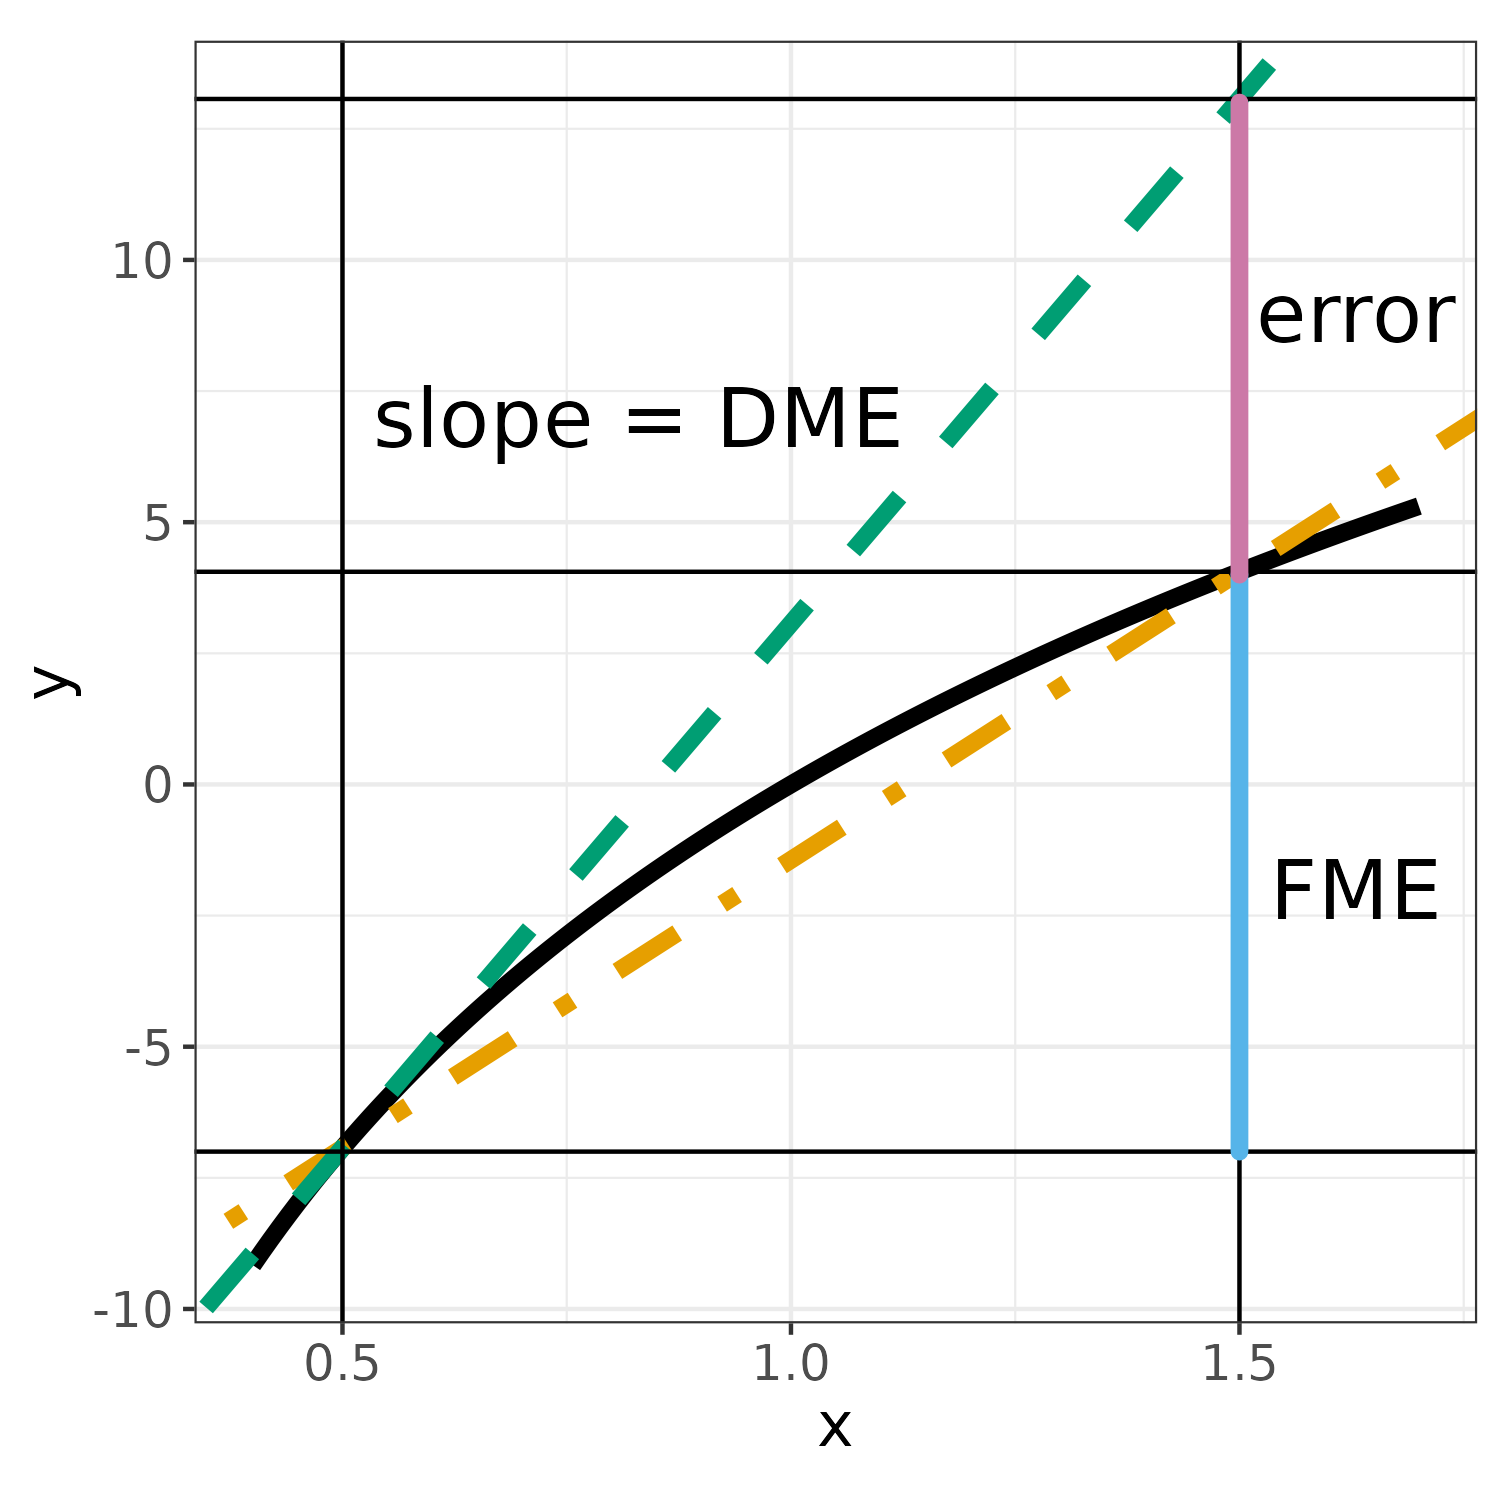
\includegraphics[width=0.8\textwidth]{figure_man/derivative_me_error.png}
% 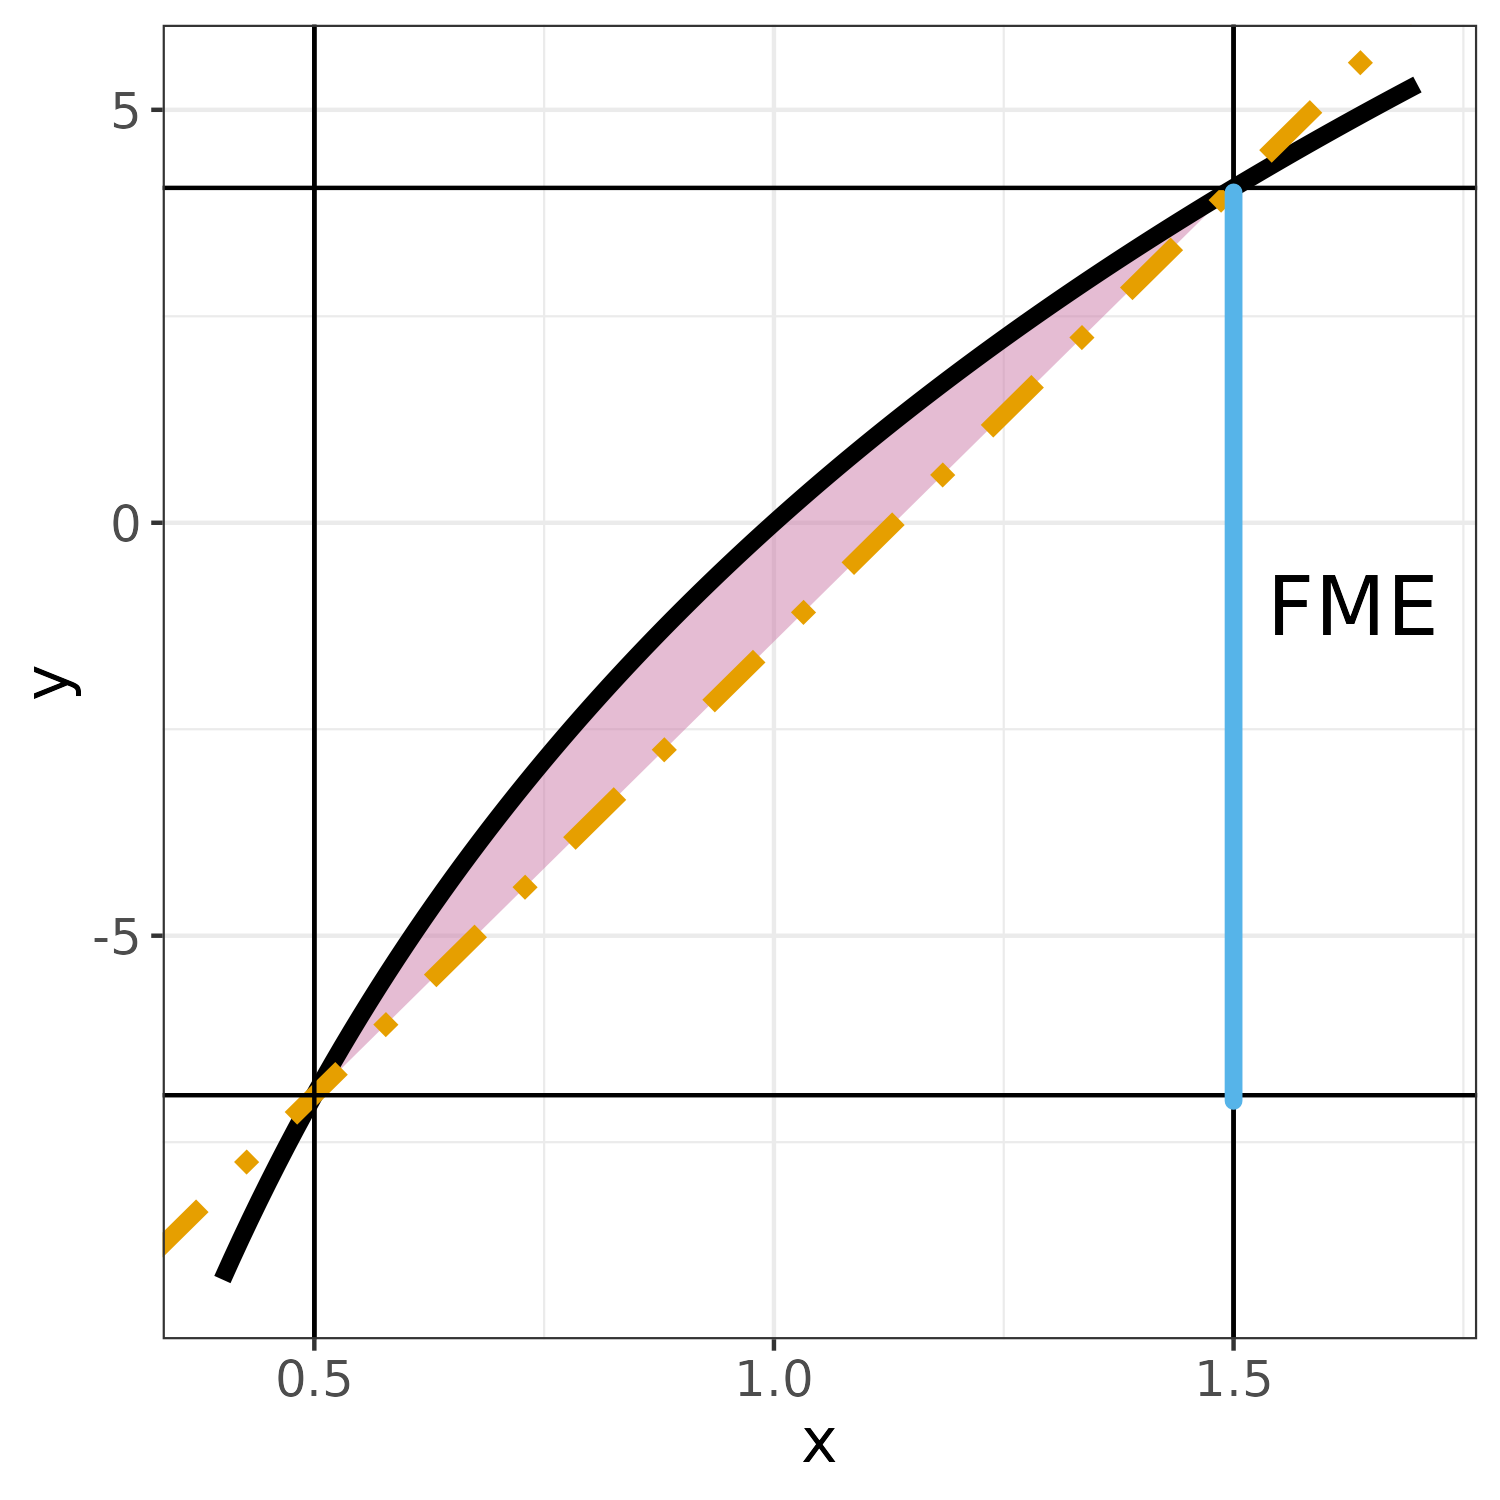
\includegraphics[width=0.8\textwidth]{figure_man/forward_me_deviation.png}
% \caption{AME fails to capture the varying effects of $X$ on $Y$ in different regions of the feature space.}
% \end{figure}
\item \textbf{Conclusion}:
\begin{itemize}
\item Need for local or regional methods like FMEs and cAMEs to capture true effects.
\end{itemize}
\end{itemize}
\end{frame}

% Forward Difference vs. Derivative
\begin{frame}{Forward Difference vs. Derivative}
\begin{columns}[T]
\begin{column}{0.65\textwidth}
\begin{itemize}
\item Derivatives of non-linear functions vary significantly at different points $\rightarrow$ DME may not be reliable.
\item FME captures the actual change in the prediction due to a finite change in the feature.
\item FME is more suitable for non-linear and non-differentiable models.
\item Both methods may lose information about the function's behavior along the change.
\item \textbf{Visualization}:
\begin{itemize}
\item DME corresponds to the slope of the tangent at a point.
\item FME corresponds to the slope of the secant between two points.
\end{itemize}
\end{itemize}
\end{column}
\begin{column}{0.35\textwidth}
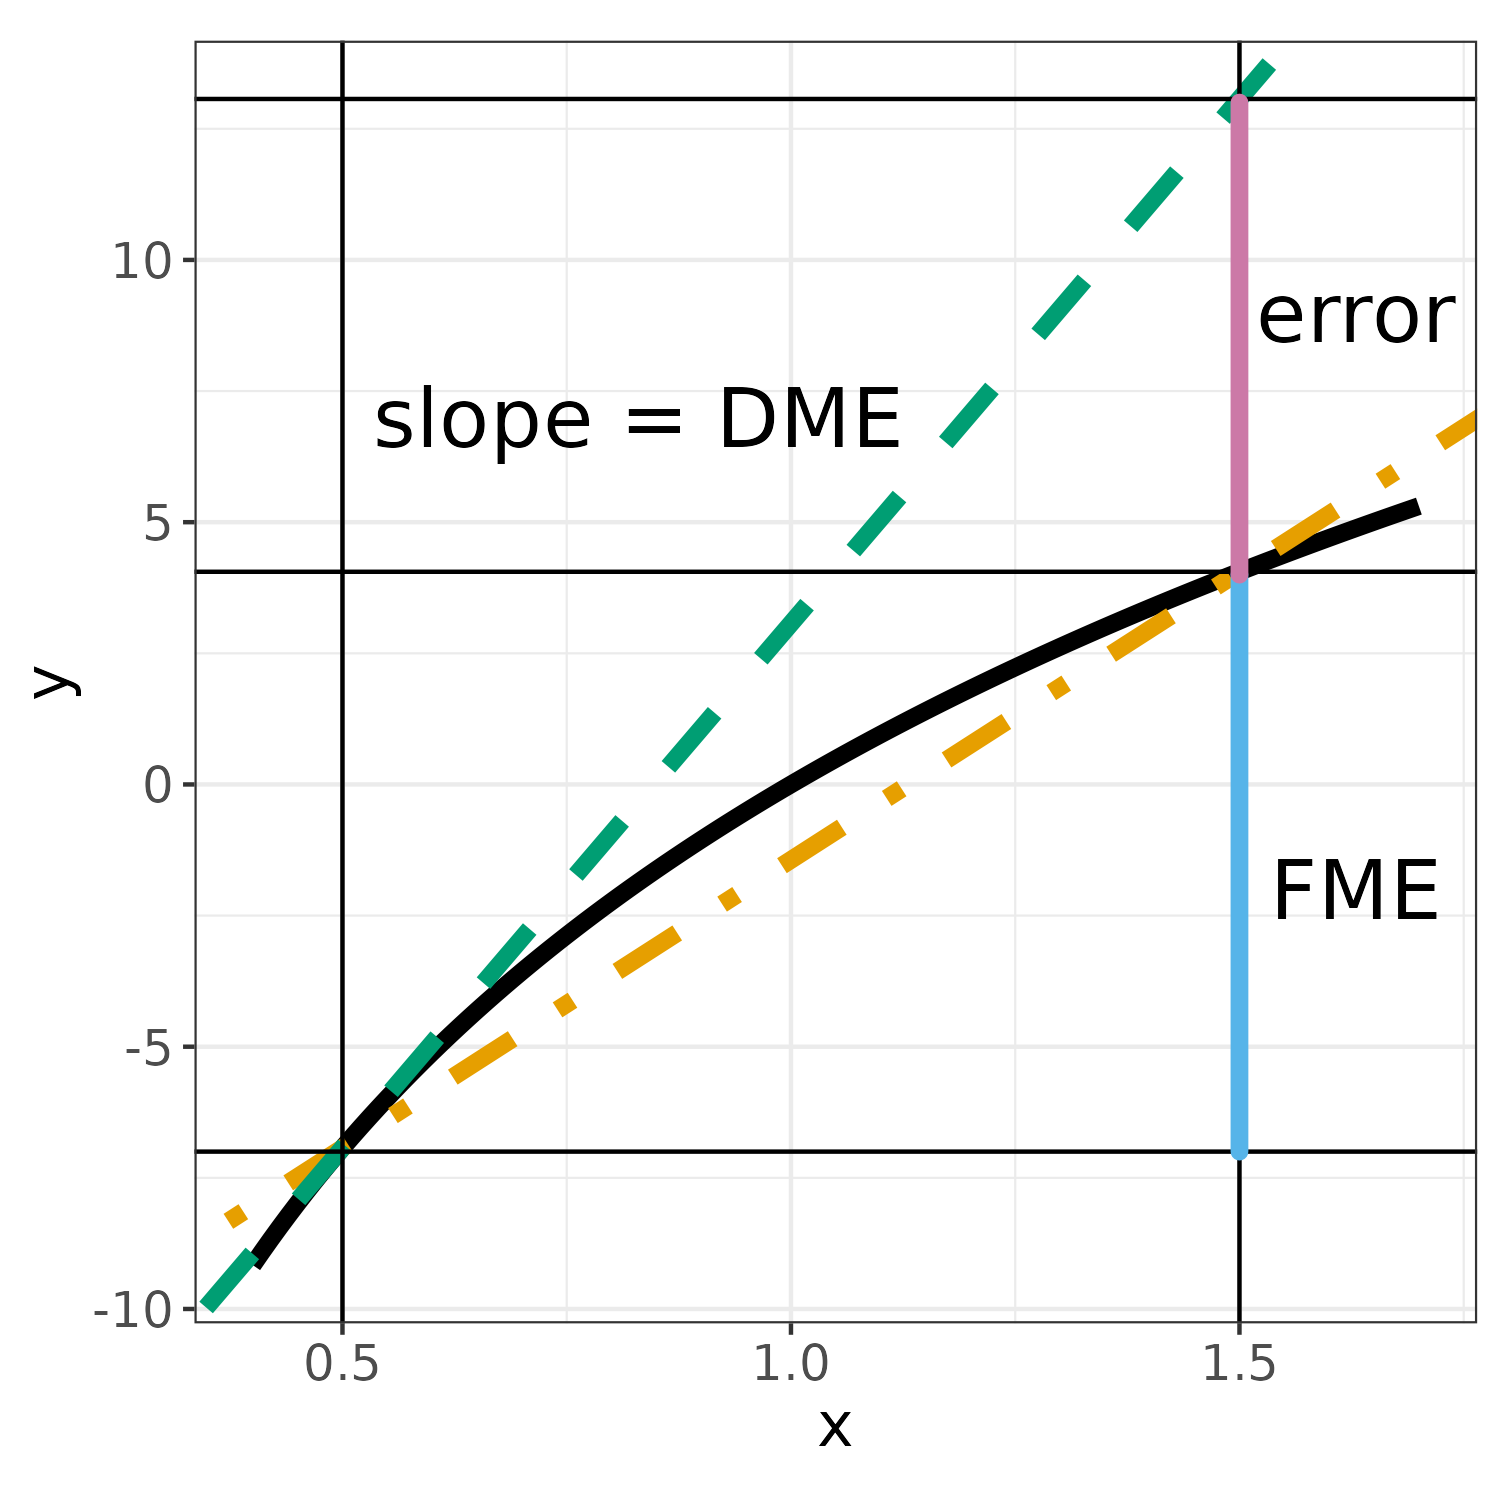
\includegraphics[width=\textwidth]{figure_man/derivative_me_error.png}
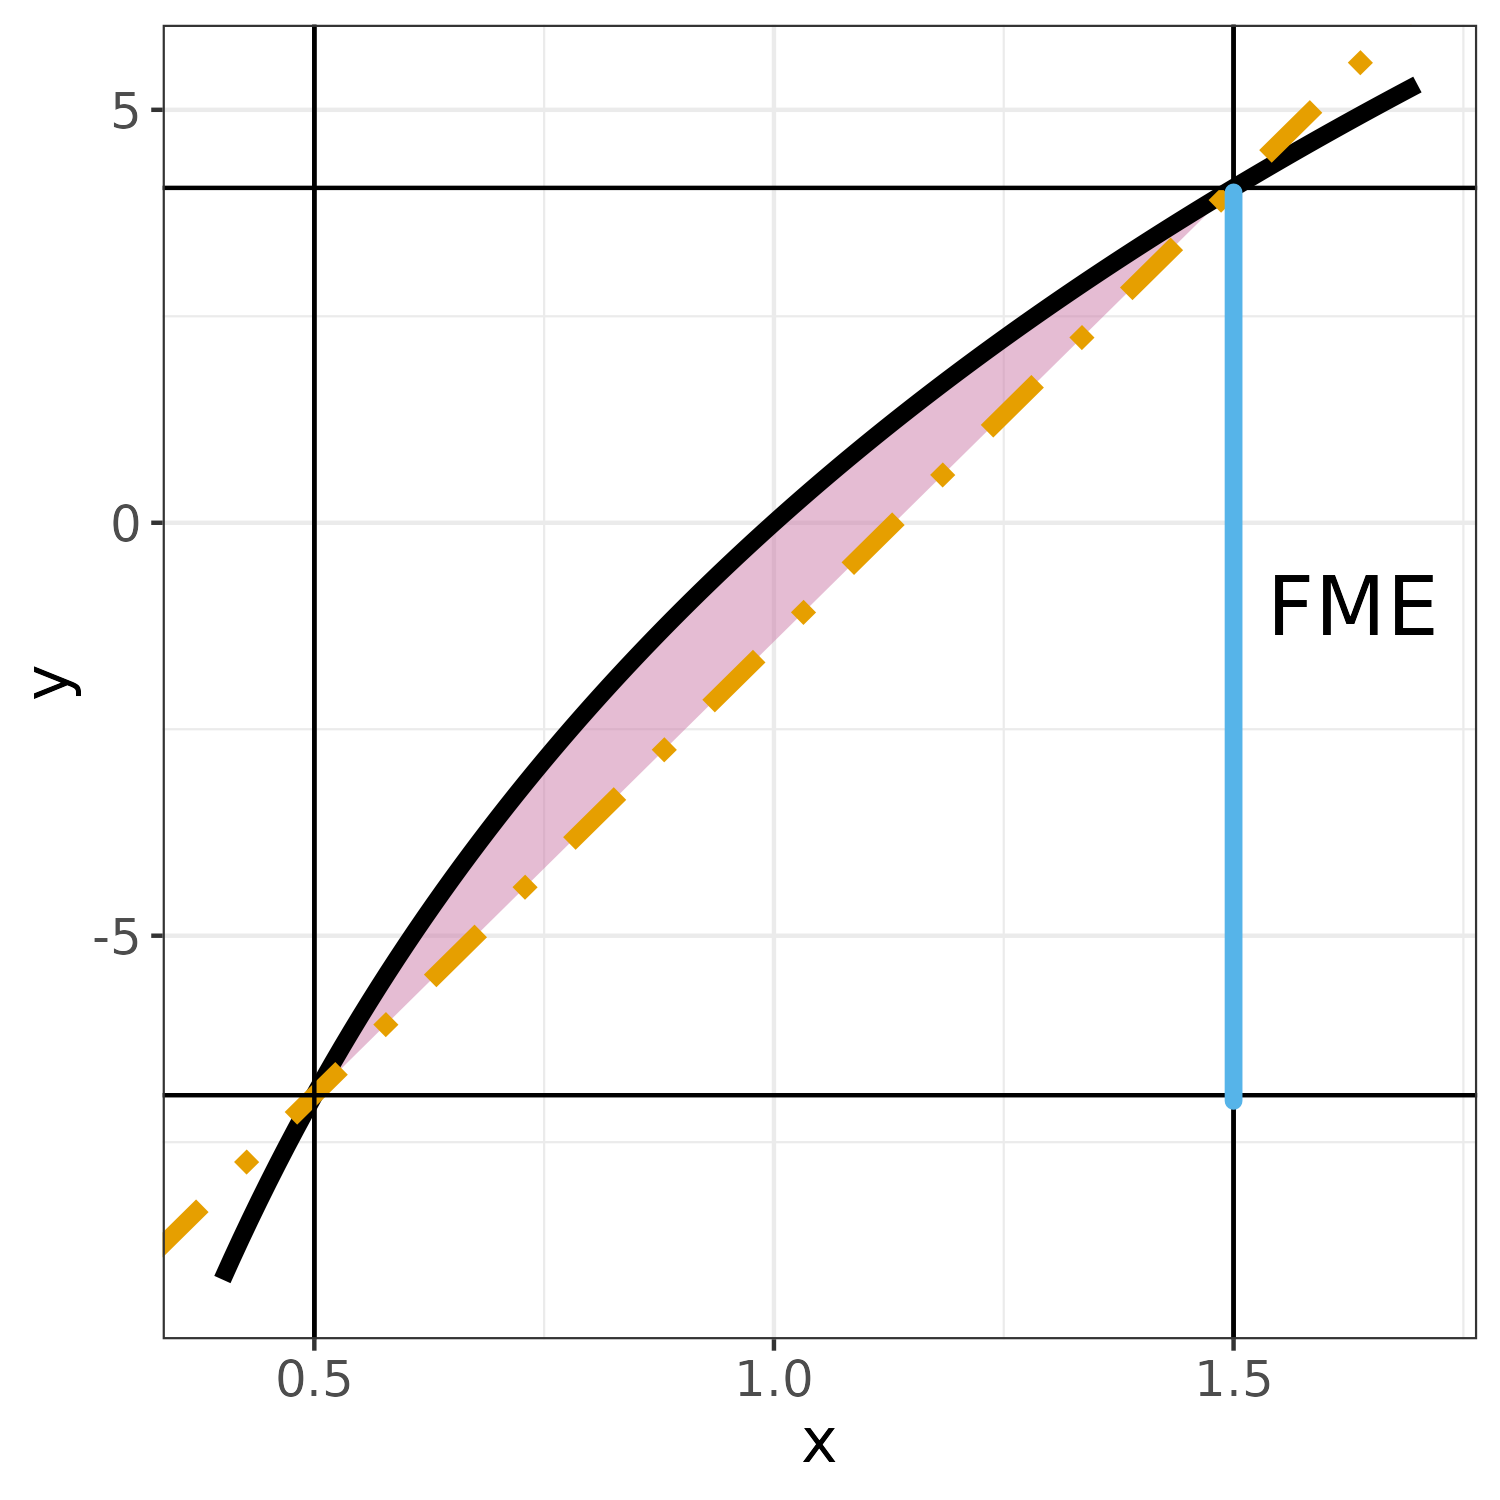
\includegraphics[width=\textwidth]{figure_man/forward_me_deviation.png}
\end{column}
\end{columns}
\end{frame}

% Additive Recovery Property
\begin{frame}{Additive Recovery Property}
\begin{itemize}
\item Both DME and FME recover only terms involving the feature(s) of interest.
\item \textbf{Example}:
\[
\widehat{f}(\xv) = a x_1 + b x_2
\]
Then:
\begin{align*}
\text{DME}_1(\xv) &= a \\
\text{FME}_1(\xv, h_1) &= a h_1
\end{align*}
\item Effects of other features linked additively are removed.
\item This property allows focusing on the direct effect of the feature.
\end{itemize}
\end{frame}

% Unified Definition of FMEs
\begin{frame}{Unified Definition of FMEs}
\begin{itemize}
\item \textbf{For Continuous Features}:
\[
\text{FME}_{\xv, \boldhS} = \widehat{f}(\xv_S + \boldhS, \xv_{-S}) - \widehat{f}(\xv)
\]
\item \textbf{For Categorical Features}:
\[
\text{FME}_{\xv, c_j} = \widehat{f}(c_j, \xv_{-j}) - \widehat{f}(\xv)
\]
\item \textbf{Mixed-Type Features}:
\begin{itemize}
\item Combine changes in both continuous and categorical features.
\end{itemize}
\item \textbf{Advantages}:
\begin{itemize}
\item Provides exact change in prediction.
\item Applicable to any model type.
\item Removes ambiguity from marginal effects definitions.
\end{itemize}
\end{itemize}
\end{frame}

%\section{Non-Linearity Measure (NLM)}

% Non-Linearity Measure (NLM)
\begin{frame}{Non-Linearity Measure (NLM)}
\begin{itemize}
\item \textbf{Purpose}:
\begin{itemize}
  \item Quantify deviation from linearity along the path of the FME.
\end{itemize}
\item \textbf{Computation}:
\begin{itemize}
  \item Compare the prediction function to the linear secant.
  \item Use the normalized integral of squared deviations.
\end{itemize}
\item \textbf{Definition}:
\[
\text{NLM}_{\xv, \boldhS} = 1 - \frac{\int_0^1 [\widehat{f}(\gamma(t)) - g_{\xv, \boldhS}(t)]^2 \Vert \gamma'(t) \Vert_2 dt}{\int_0^1 [\widehat{f}(\gamma(t)) - \overline{\widehat{f}}]^2 \Vert \gamma'(t) \Vert_2 dt}
\]
\item \textbf{Interpretation}:
\begin{itemize}
  \item NLM $\in (-\infty, 1]$.
  \item NLM $=1$: Perfect linearity.
  \item NLM $\leq 0$: Indicates strong non-linearity.
\end{itemize}
\end{itemize}
\end{frame}

% Computation and Interpretation of NLM
\begin{frame}{Computation and Interpretation of NLM}
\begin{itemize}
\item \textbf{Linear Reference Function}:
\[
g_{\xv, \boldhS}(t) = \widehat{f}(\xv) + t \cdot \text{FME}_{\xv, \boldhS}
\]
\item \textbf{Path Parameterization}:
\[
\gamma(t) = \xv + t \cdot \boldhS
\]
\item \textbf{Line Integrals}:
\begin{align*}
\text{(I)} &= \int_0^1 [\widehat{f}(\gamma(t)) - g_{\xv, \boldhS}(t)]^2 \Vert \boldhS \Vert_2 dt \\
\text{(II)} &= \int_0^1 [\widehat{f}(\gamma(t)) - \overline{\widehat{f}}]^2 \Vert \boldhS \Vert_2 dt
\end{align*}
\item \textbf{Advantages}:
\begin{itemize}
\item Provides a quantitative measure of non-linearity.
\item Applicable to univariate and multivariate feature changes.
\item Helps assess the reliability of linear approximations.
\end{itemize}
\end{itemize}
\end{frame}

% Visualization of NLM
\begin{frame}{Visualization of NLM}
\begin{figure}
  \centering
  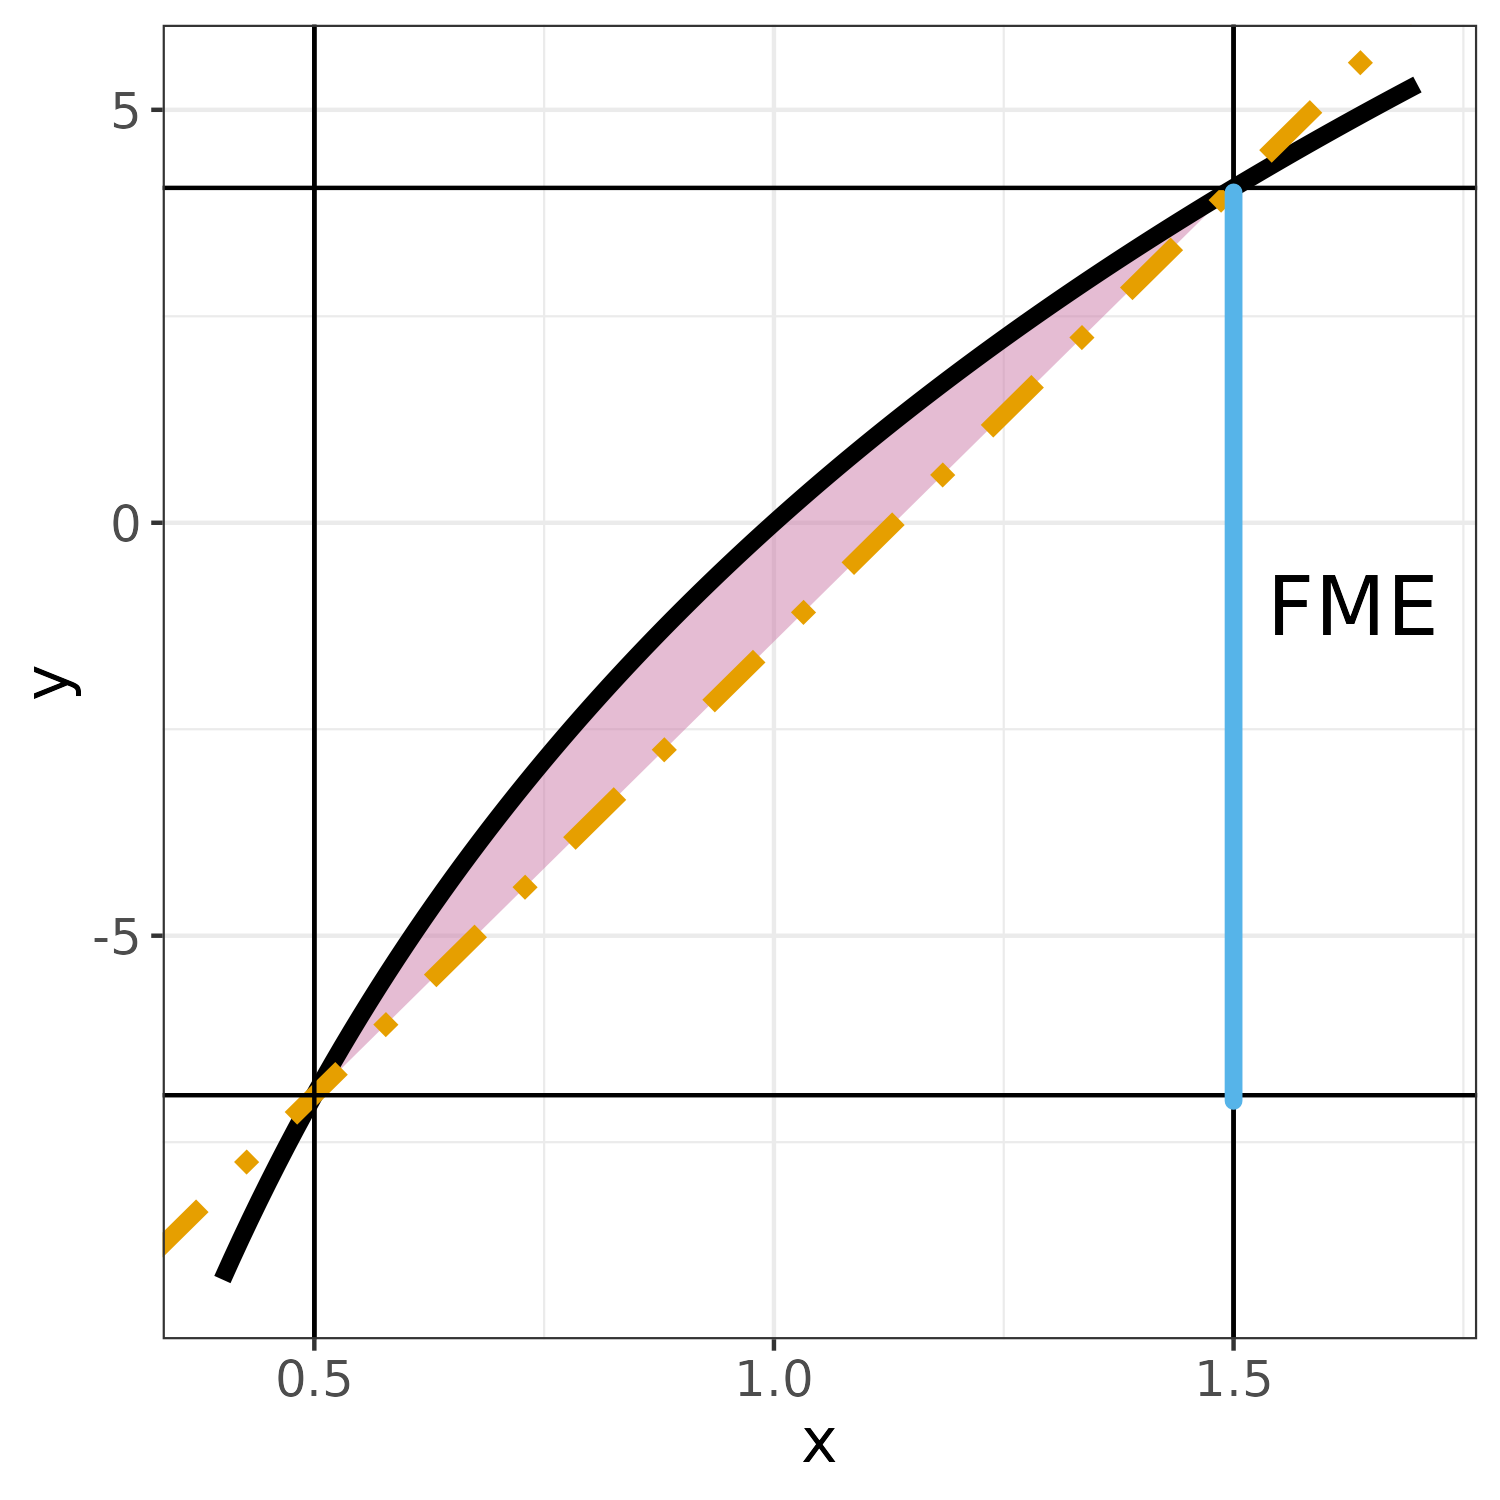
\includegraphics[width=0.6\textwidth]{figure_man/forward_me_deviation.png}
  \caption{Comparison between the prediction function and the linear secant. The purple area represents the deviation quantified by the NLM.}
\end{figure}
\end{frame}

%\section{Selecting Step Sizes and Trust Regions}

% Selecting Step Sizes and Trust Regions
\begin{frame}{Selecting Step Sizes and Trust Regions}
\begin{itemize}
\item \textbf{Step Size Selection}:
\begin{itemize}
  \item Based on domain knowledge or natural units.
  \item Use statistical measures (e.g., standard deviation, IQR).
  \item Contextual information dictates meaningful step sizes.
\end{itemize}
\item \textbf{Local Linear Trust Region (LLTR)}:
\begin{itemize}
  \item Identify regions where NLM indicates approximate linearity (e.g., NLM $\geq 0.9$).
  \item Allows for reliable interpretation of FMEs.
  \item Step sizes within LLTR ensure linear approximation is valid.
\end{itemize}
\end{itemize}
\end{frame}

% LLTR Visualization
\begin{frame}{Local Linear Trust Region (LLTR) Visualization}
\begin{figure}
  \centering
  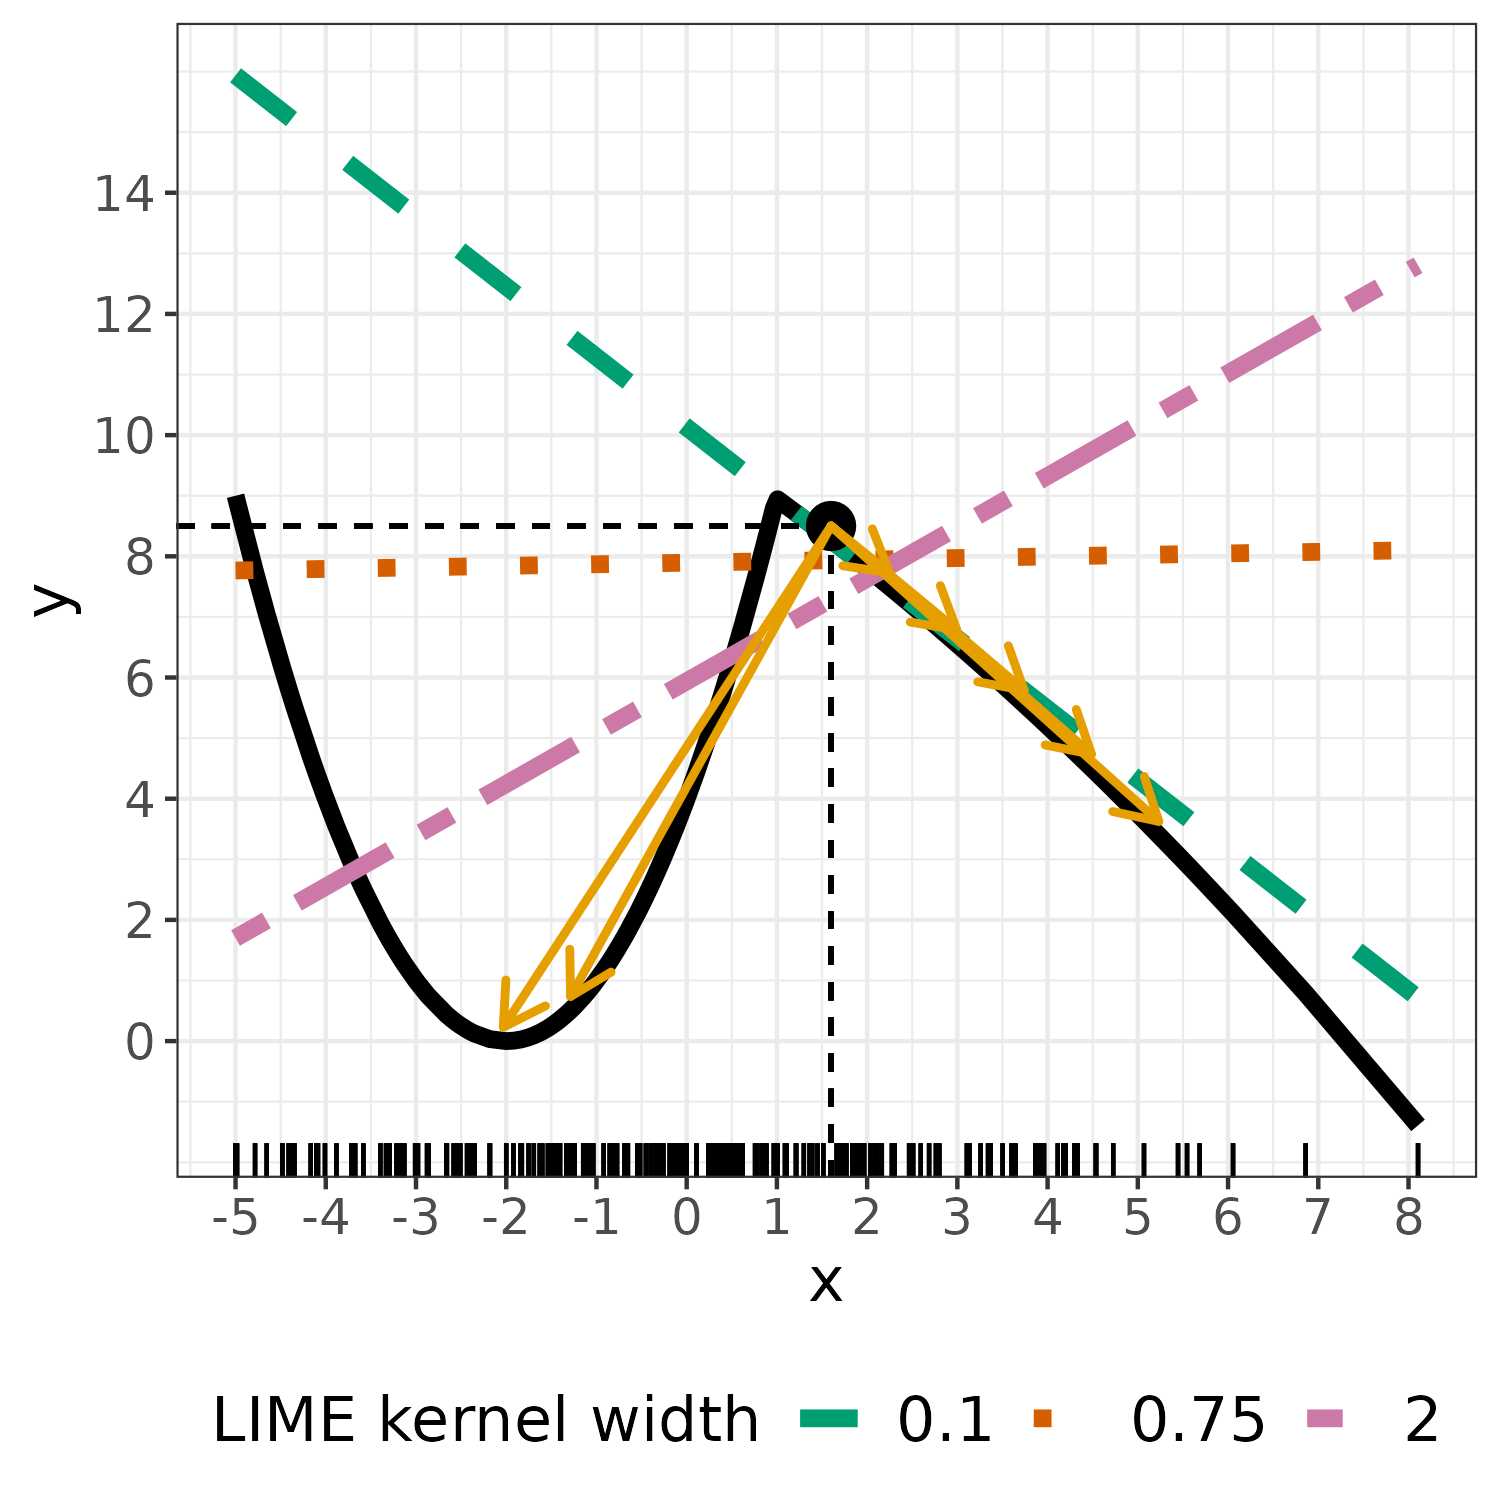
\includegraphics[width=0.6\textwidth]{figure_man/fme_trust_region_lime.png}
  \caption{LLTR using FMEs compared to LIME explanations. The orange arrows represent steps where NLM indicates linearity.}
\end{figure}
\end{frame}

% Model Extrapolation and Step Sizes
\begin{frame}{Model Extrapolation and Step Sizes}
\begin{itemize}
\item \textbf{Model Extrapolation Risks}:
\begin{itemize}
\item Large step sizes may lead to extrapolation beyond the training data.
\item Predictions in extrapolated regions may be unreliable.
\end{itemize}
\item \textbf{Mitigation}:
\begin{itemize}
\item Limit step sizes to ranges within the training data.
\item Identify and exclude extrapolation points (EPs) from analysis.
\end{itemize}
\item \textbf{Visualization}:
\begin{figure}
  \centering
  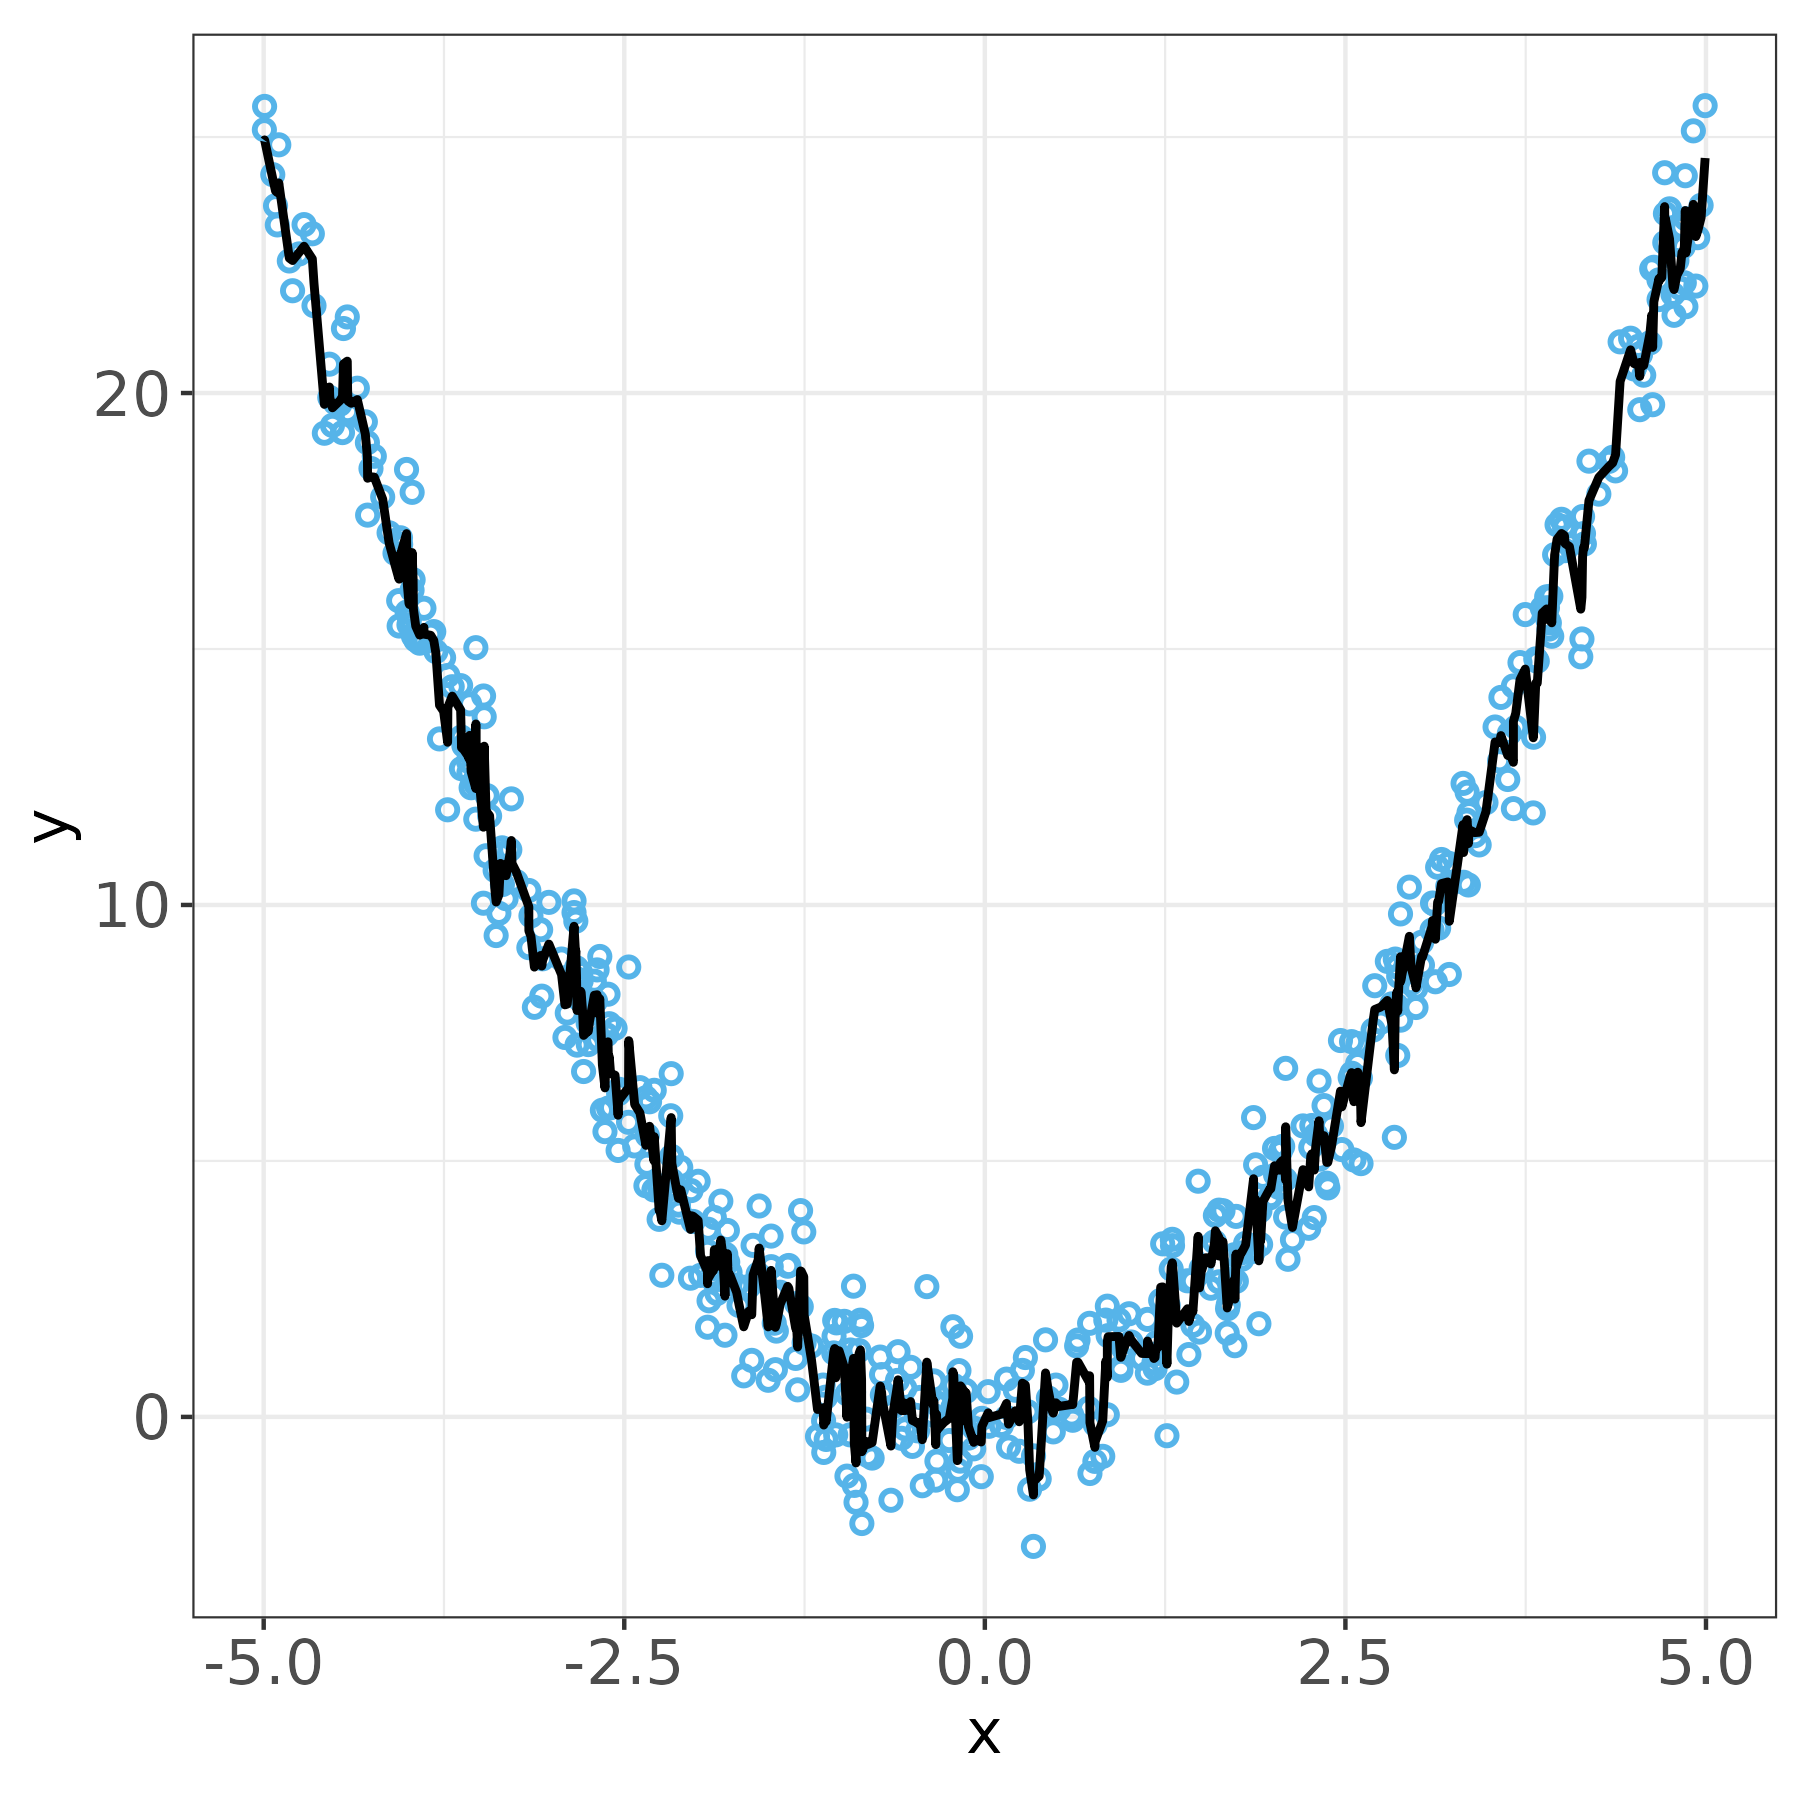
\includegraphics[width=0.5\textwidth]{figure_man/uniform_extrapolation_data.png}
  \caption{Model extrapolation occurs when moving beyond the training data range.}
\end{figure}
\end{itemize}
\end{frame}

%\section{Conditional Average Marginal Effects (cAMEs)}

% Conditional Average Marginal Effects (cAMEs)
\begin{frame}{Conditional Average Marginal Effects (cAMEs)}
\begin{itemize}
\item \textbf{Purpose}:
\begin{itemize}
\item Estimate expected FMEs within specific subgroups or regions.
\item Capture regional effects in non-linear models.
\end{itemize}
\item \textbf{Definition}:
\[
\text{cAME}_{\mathcal{D}_{[\;]}, \boldhS} = \frac{1}{n_{[\;]}} \sum_{i \,:\, \xv^{(i)} \in \mathcal{D}_{[\;]}} \left[ \widehat{f}\left(\xv_S^{(i)} + \boldhS, \xv_{-S}^{(i)}\right) - \widehat{f}\left(\xv^{(i)}\right) \right]
\]
\item \textbf{Subgroups}:
\begin{itemize}
\item Defined based on feature values or characteristics.
\item Aim to have homogeneous effects within subgroups.
\end{itemize}
\end{itemize}
\end{frame}

% Desiderata for Finding Subgroups
\begin{frame}{Desiderata for Finding Subgroups}
\begin{itemize}
\item \textbf{Within-Group Effect Homogeneity}:
\begin{itemize}
\item Minimize FME variance within subgroups.
\end{itemize}
\item \textbf{Between-Group Effect Heterogeneity}:
\begin{itemize}
\item Maximize differences in cAMEs between subgroups.
\end{itemize}
\item \textbf{Full Segmentation}:
\begin{itemize}
\item Entire dataset is partitioned into subgroups.
\end{itemize}
\item \textbf{Non-Congruence}:
\begin{itemize}
\item Subgroups do not overlap.
\end{itemize}
\item \textbf{Confidence and Stability}:
\begin{itemize}
\item Prefer larger, stable subgroups.
\item Subgroups should be consistent across data variations.
\end{itemize}
\end{itemize}
\end{frame}

% Estimation Using Decision Trees
\begin{frame}{Estimation Using Decision Trees}
\begin{itemize}
\item \textbf{Recursive Partitioning (RP)}:
\begin{itemize}
\item Use decision trees to partition the feature space.
\item Find subgroups with homogeneous FMEs.
\end{itemize}
\item \textbf{Conditional Inference Trees (CTREE)}:
\begin{itemize}
\item Use statistical tests to find significant splits.
\item Help stabilize the splits and improve subgroup reliability.
\end{itemize}
\item \textbf{Advantages}:
\begin{itemize}
\item Automatically identify meaningful subgroups.
\item Handle complex interactions and non-linearities.
\end{itemize}
\end{itemize}
\end{frame}

% Confidence Intervals for cAME and cANLM
\begin{frame}{Confidence Intervals for cAME and cANLM}
\begin{itemize}
\item \textbf{Purpose}:
\begin{itemize}
\item Provide uncertainty estimates for cAMEs and cANLMs.
\end{itemize}
\item \textbf{Computation}:
\begin{align*}
\text{CI}_{\text{cAME}, \; 1 - \alpha} &= \left[\text{cAME}_{\mathcal{D}_{[\;]}, \boldhS} \pm t_{1-\frac{\alpha}{2}, n_{[\;]}-1} \frac{\text{SD}_{\text{FME}, [\;]}}{\sqrt{n_{[\;]}}} \right] \\
\text{CI}_{\text{cANLM}, \; 1 - \alpha} &= \left[\text{cANLM}_{\mathcal{D}_{[\;]}, \boldhS} \pm t_{1-\frac{\alpha}{2}, n_{[\;]}-1} \frac{\text{SD}_{\text{NLM}, [\;]}}{\sqrt{n_{[\;]}}} \right]
\end{align*}
\item \textbf{Interpretation}:
\begin{itemize}
\item Narrow intervals indicate higher confidence.
\item Larger subgroups provide more reliable estimates.
\end{itemize}
\end{itemize}
\end{frame}

%\section{Related Work}

% Relation to ICE and PD
\begin{frame}{Relation to ICE and PD}
\begin{itemize}
\item \textbf{Individual Conditional Expectation (ICE)}:
\begin{itemize}
\item Visualizes predictions for an observation across a range of feature values.
\item FME corresponds to vertical differences between points on an ICE curve.
\end{itemize}
\item \textbf{Partial Dependence (PD)}:
\begin{itemize}
\item Shows average predictions across a range of feature values.
\item AME is equivalent to vertical differences on PD for linear models.
\end{itemize}
\item \textbf{Advantages of FMEs}:
\begin{itemize}
\item Provide exact change in prediction.
\item Applicable to high-dimensional feature changes.
\item Quantifiable and not limited to visual interpretation.
\end{itemize}
\end{itemize}
\end{frame}

% Comparison to LIME
\begin{frame}{Comparison to LIME}
\begin{itemize}
\item \textbf{LIME (Local Interpretable Model-Agnostic Explanations)}:
\begin{itemize}
\item Trains a local surrogate model around an observation.
\item Interpretation depends on surrogate model parameters.
\end{itemize}
\item \textbf{Differences with FMEs}:
\begin{itemize}
\item FMEs directly compute changes without surrogates.
\item FMEs are deterministic with fixed parameters.
\item LIME explanations can vary due to randomness and parameter choices.
\end{itemize}
\item \textbf{Advantages of FMEs}:
\begin{itemize}
\item More stable and interpretable.
\item NLM provides measure of linearity and trust in the explanation.
\end{itemize}
\end{itemize}
\end{frame}

% Sensitivity Analysis
\begin{frame}{Relation to Sensitivity Analysis}
\begin{itemize}
\item \textbf{Purpose of Sensitivity Analysis (SA)}:
\begin{itemize}
\item Determine how uncertainty in model output can be attributed to inputs.
\end{itemize}
\item \textbf{Methods in SA}:
\begin{itemize}
\item Use finite differences to estimate local sensitivities.
\item Elementary effects correspond to univariate forward difference quotients.
\end{itemize}
\item \textbf{Relation to FMEs}:
\begin{itemize}
\item FMEs can be seen as a form of sensitivity analysis.
\item Provide insight into feature importance and interactions.
\end{itemize}
\end{itemize}
\end{frame}

%\section{Conclusion}

% Conclusion and Future Work
\begin{frame}{Conclusion and Future Work}
\begin{itemize}
\item \textbf{Key Takeaways}:
\begin{itemize}
  \item FMEs provide exact changes in predictions for any model type.
  \item NLM helps assess the linearity of effects along feature changes.
  \item cAMEs enable regional interpretations, capturing heterogeneity.
  \item Unified approach removes ambiguity from marginal effects.
\end{itemize}
\item \textbf{Future Directions}:
\begin{itemize}
  \item Enhance methods for detecting model extrapolations.
  \item Explore stabilization techniques for subgroup discovery.
  \item Investigate applications of FMEs in feature importance and other domains.
  \item Integrate FMEs with other interpretability methods.
\end{itemize}
\end{itemize}
\end{frame}


% References (if needed)
% \begin{frame}[allowframebreaks]{References}
% \bibliographystyle{apalike}
% \bibliography{references}
% \end{frame}

\endlecture
\end{document}
